% !TEX root = mythesis.tex

%==============================================================================
\chapter{Results}
\label{sec:results}
%==============================================================================
The aim of this chapter is to present the final results of the multijet estimate using the ABCD method, including all the uncertainties discussed in the previous chapter. A performance comparison with the use of different taggers on the multijet estimation is shown in section \ref{sec:results:taggers}. A similar kind of performance comparison is also studied by using different jet collections, which is described in section \ref{sec:results:jetcollections}.
 
%==============================================================================
\section{Estimated multijet including uncertainties}
\label{sec:results:estimation}
%==============================================================================
The multijet estimate in the validation region using the ABCD method, including all the discussed uncertainties is shown in Fig.\ \ref{fig:results:estimation}. It shows the estimated multijet in all the six kinematic distributions where each distribution is having different event yields and different uncertainties. The difference between the estimated multijet (and other backgrounds) and the data is within the described uncertainty. In Fig.\ \ref{fig:results:estimation:jet_pt}, the significant amount of uncertainty can be seen in \pt distribution of the leading $b$-jet because of the shape uncertainty, which is primarily from the closure uncertainty as discussed in section \ref{sec:uncertainties:systematics:closure}. A similar kind of behaviour can also be seen in the mass distributions. Table \ref{table:results:estimation} shows the event yield of the estimated multijet along with their uncertainties for all the distributions. It can be observed that the multijet (from the ABCD method) plus the contribution from other backgrounds (from the MC simulation) agree well with the data within the described uncertainties.

\begin{table}[hbt!]
	\centering
	\begin{tabular}{c|c|c} 
		\toprule
		Distribution & Event yield & Plots\\ 
		\midrule
		$W$-tagged jet \pt & $\num{72071} \pm \num{288} \text{ (stat.)} \pm \num{2745} \text{ (sys.)}$ & Fig.\ \ref{fig:results:estimation:ljet_pt} \\
		$W$-tagged jet mass & $\num{72752} \pm \num{363} \text{ (stat.)} \pm \num{4765} \text{ (sys.)}$ & Fig.\ \ref{fig:results:estimation:ljet_m} \\
		$W$-tagged jet $\eta$ & $\num{72613} \pm \num{290} \text{ (stat.)} \pm \num{3199} \text{ (sys.)}$ & Fig.\ \ref{fig:results:estimation:ljet_eta} \\
		leading $b$-tagged jet \pt & $\num{71669} \pm \num{1863} \text{ (stat.)} \pm \num{7245} \text{ (sys.)}$ & Fig.\ \ref{fig:results:estimation:jet_pt} \\
		leading $b$-tagged jet mass & $\num{73038} \pm \num{292} \text{ (stat.)} \pm \num{3488} \text{ (sys.)}$ & Fig.\ \ref{fig:results:estimation:jet_m} \\
		VLQ mass & $\num{72572} \pm \num{580} \text{ (stat.)} \pm \num{3343} \text{ (sys.)}$ & Fig.\ \ref{fig:results:estimation:VLQM} \\
		\midrule
		Other bkg.\ & $\num{3320} \pm \num{95} \text{ (stat.)}$ & \\ 
		\midrule
		\textbf{Data} & \textbf{\num{75967}} & \\
		\bottomrule
	\end{tabular}
	\caption{Result showing the estimated multijet with all the uncertainties in the validation region for all the kinematic distributions.}
	\label{table:results:estimation}
\end{table}


\begin{figure}[hbt!]
	\centering
	\graphicspath{{figs/chapter6/final/}}
	\begin{subfigure}{.35\textwidth}
		\centering
		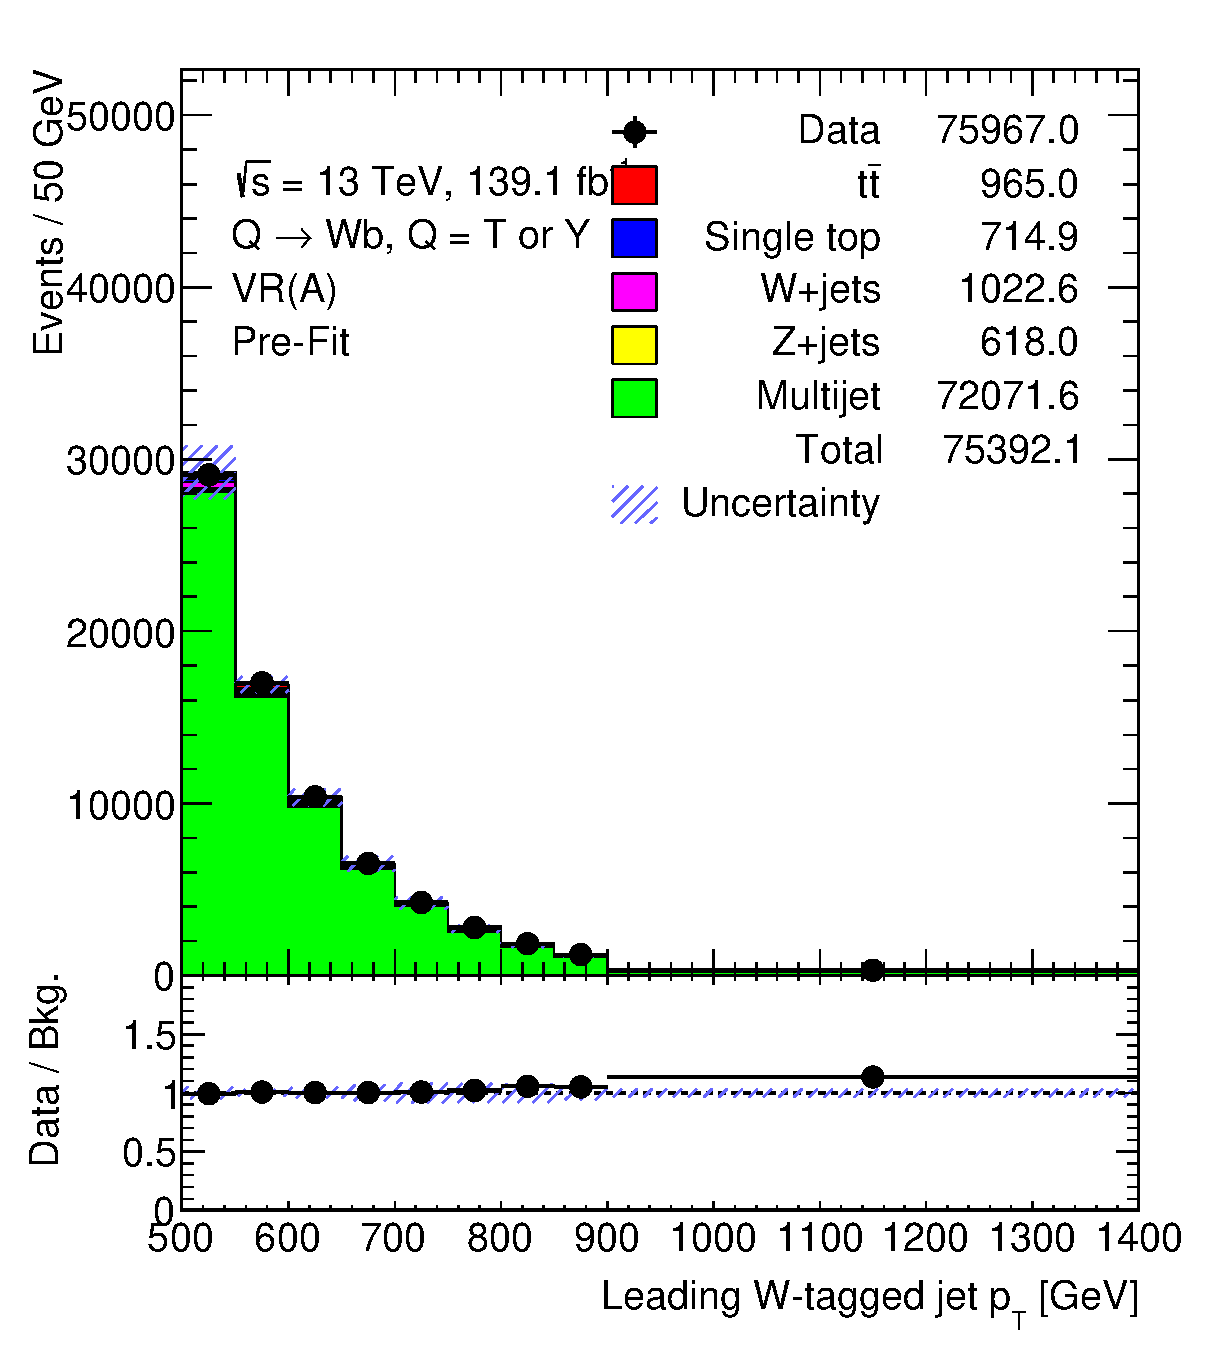
\includegraphics[width=\linewidth,height=\textheight,keepaspectratio]{VR_B_ljet_pt.eps}
		\caption{}
		\label{fig:results:estimation:ljet_pt}
	\end{subfigure}\hspace{0.6cm}
	\begin{subfigure}{.35\textwidth}
		\centering
		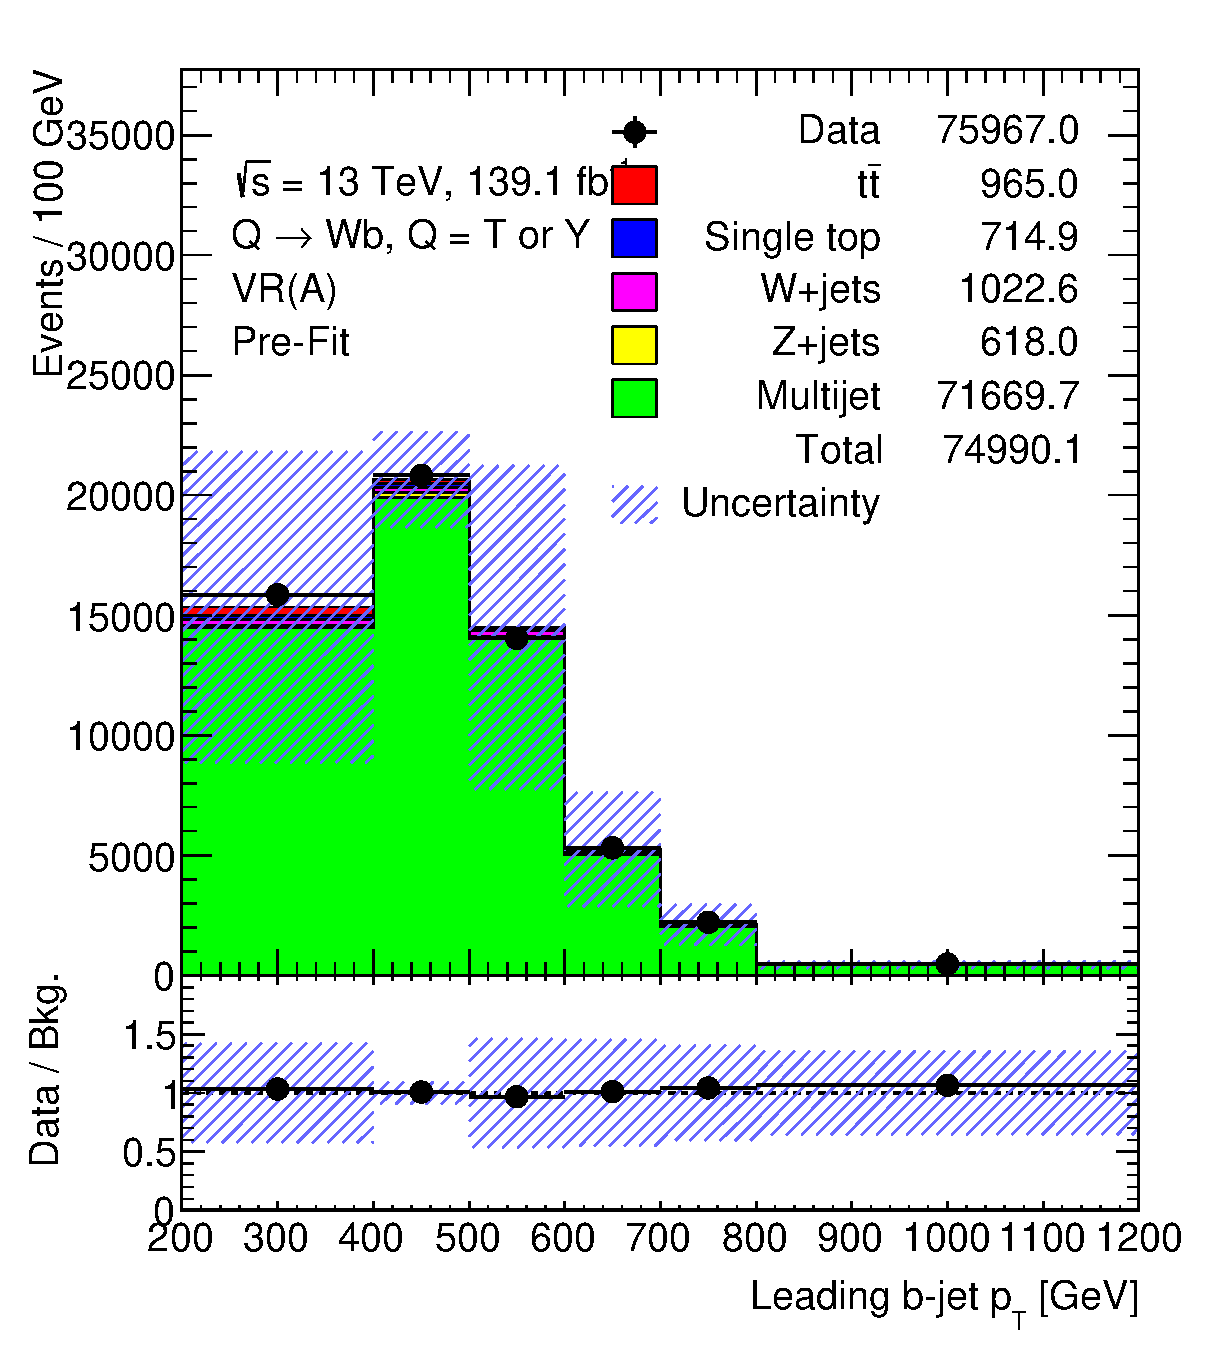
\includegraphics[width=\linewidth,height=\textheight,keepaspectratio]{VR_B_jet_pt.eps}
		\caption{}
		\label{fig:results:estimation:jet_pt}
	\end{subfigure}
	\begin{subfigure}{.35\textwidth}
		\centering
		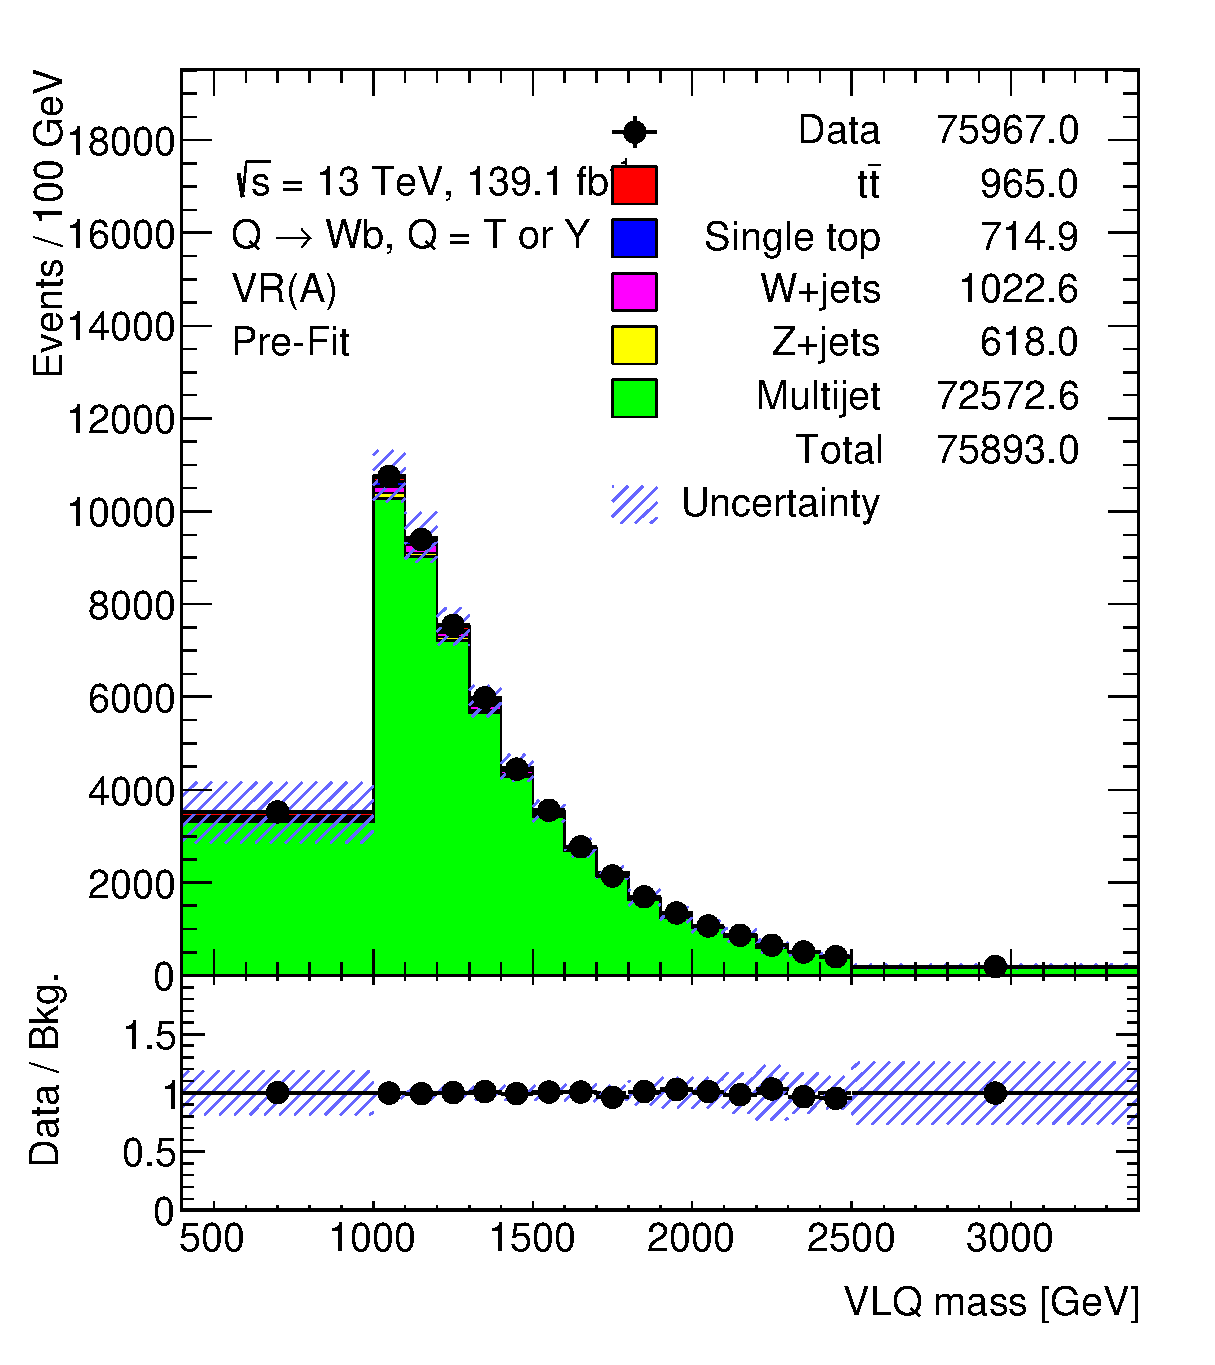
\includegraphics[width=\linewidth,height=\textheight,keepaspectratio]{VR_B_VLQM.eps}
		\caption{}
		\label{fig:results:estimation:VLQM}
	\end{subfigure}\hspace{0.6cm}
	\begin{subfigure}{.35\textwidth}
		\centering
		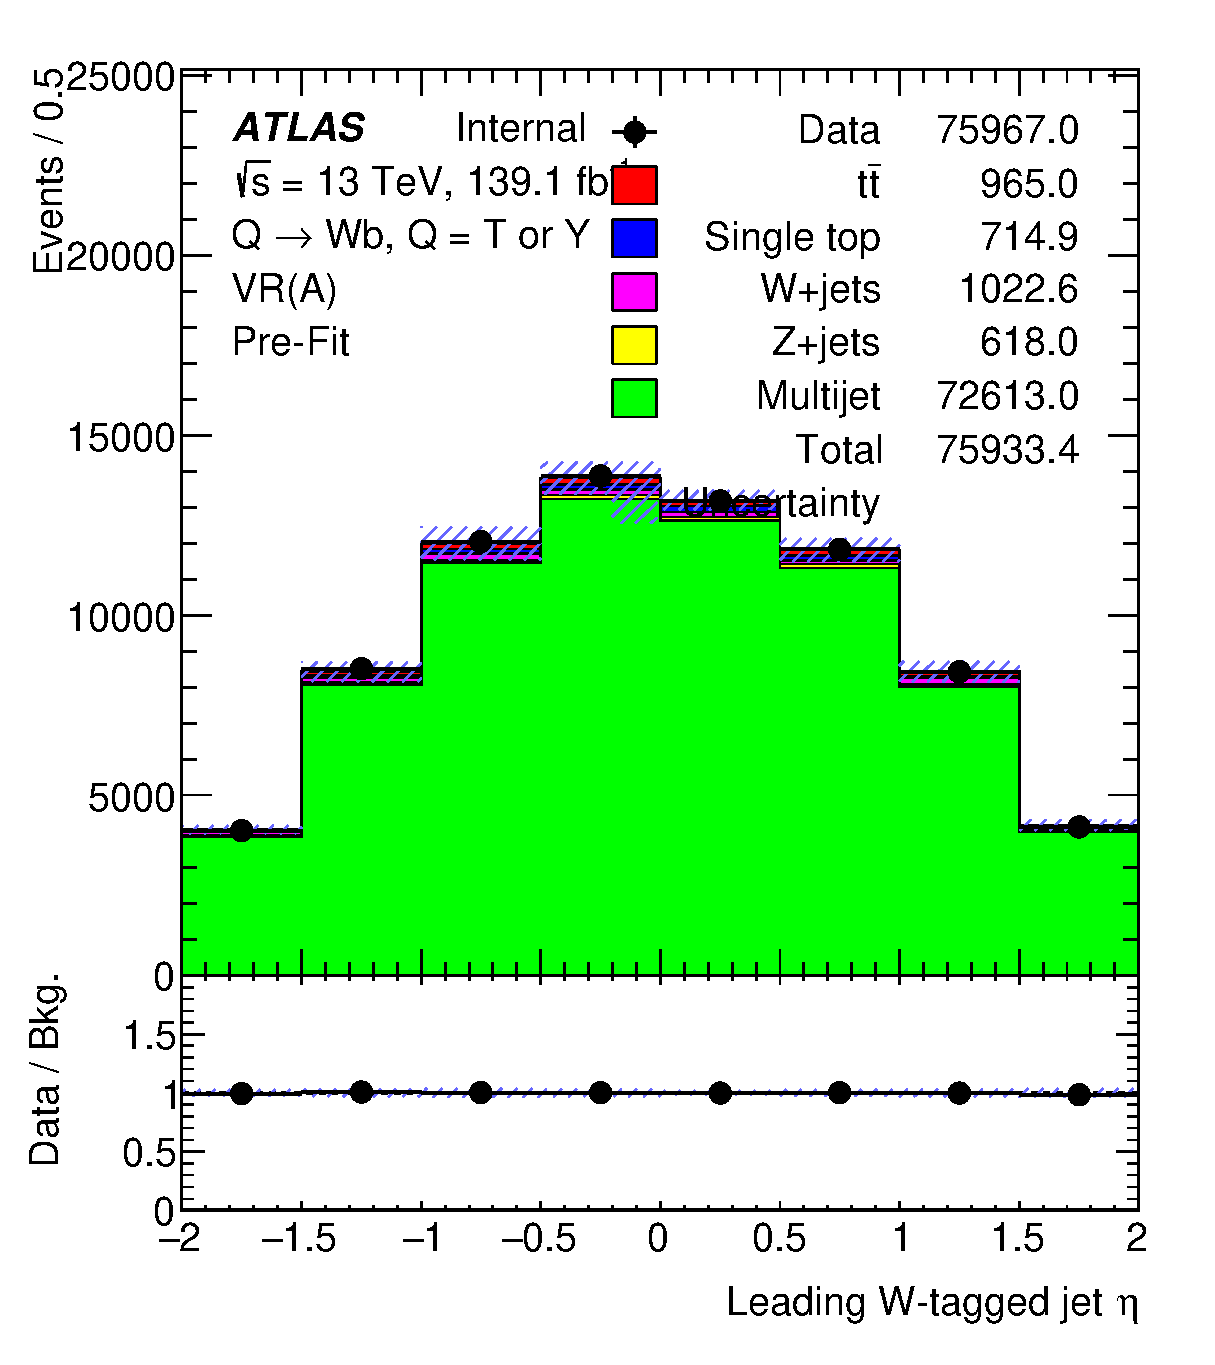
\includegraphics[width=\linewidth,height=\textheight,keepaspectratio]{VR_B_ljet_eta.eps}
		\caption{}
		\label{fig:results:estimation:ljet_eta}
	\end{subfigure}
	\begin{subfigure}{.35\textwidth}
		\centering
		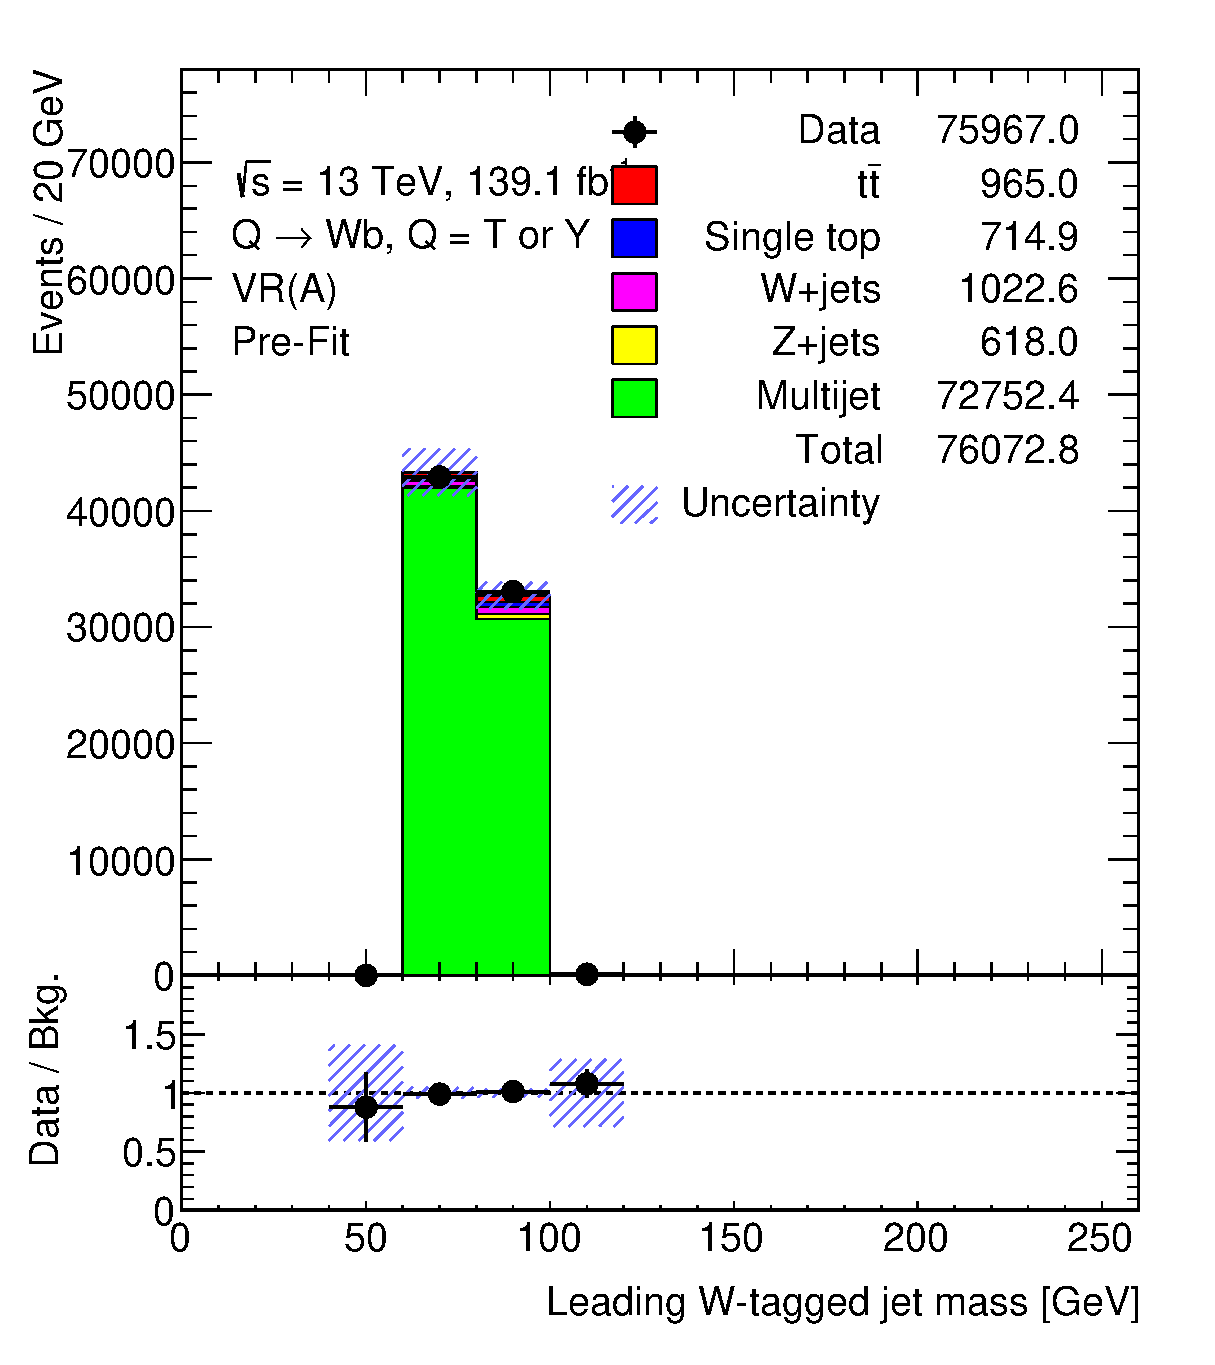
\includegraphics[width=\linewidth,height=\textheight,keepaspectratio]{VR_B_ljet_m.eps}
		\caption{}
		\label{fig:results:estimation:ljet_m}
	\end{subfigure}\hspace{0.6cm}
	\begin{subfigure}{.35\textwidth}
		\centering
		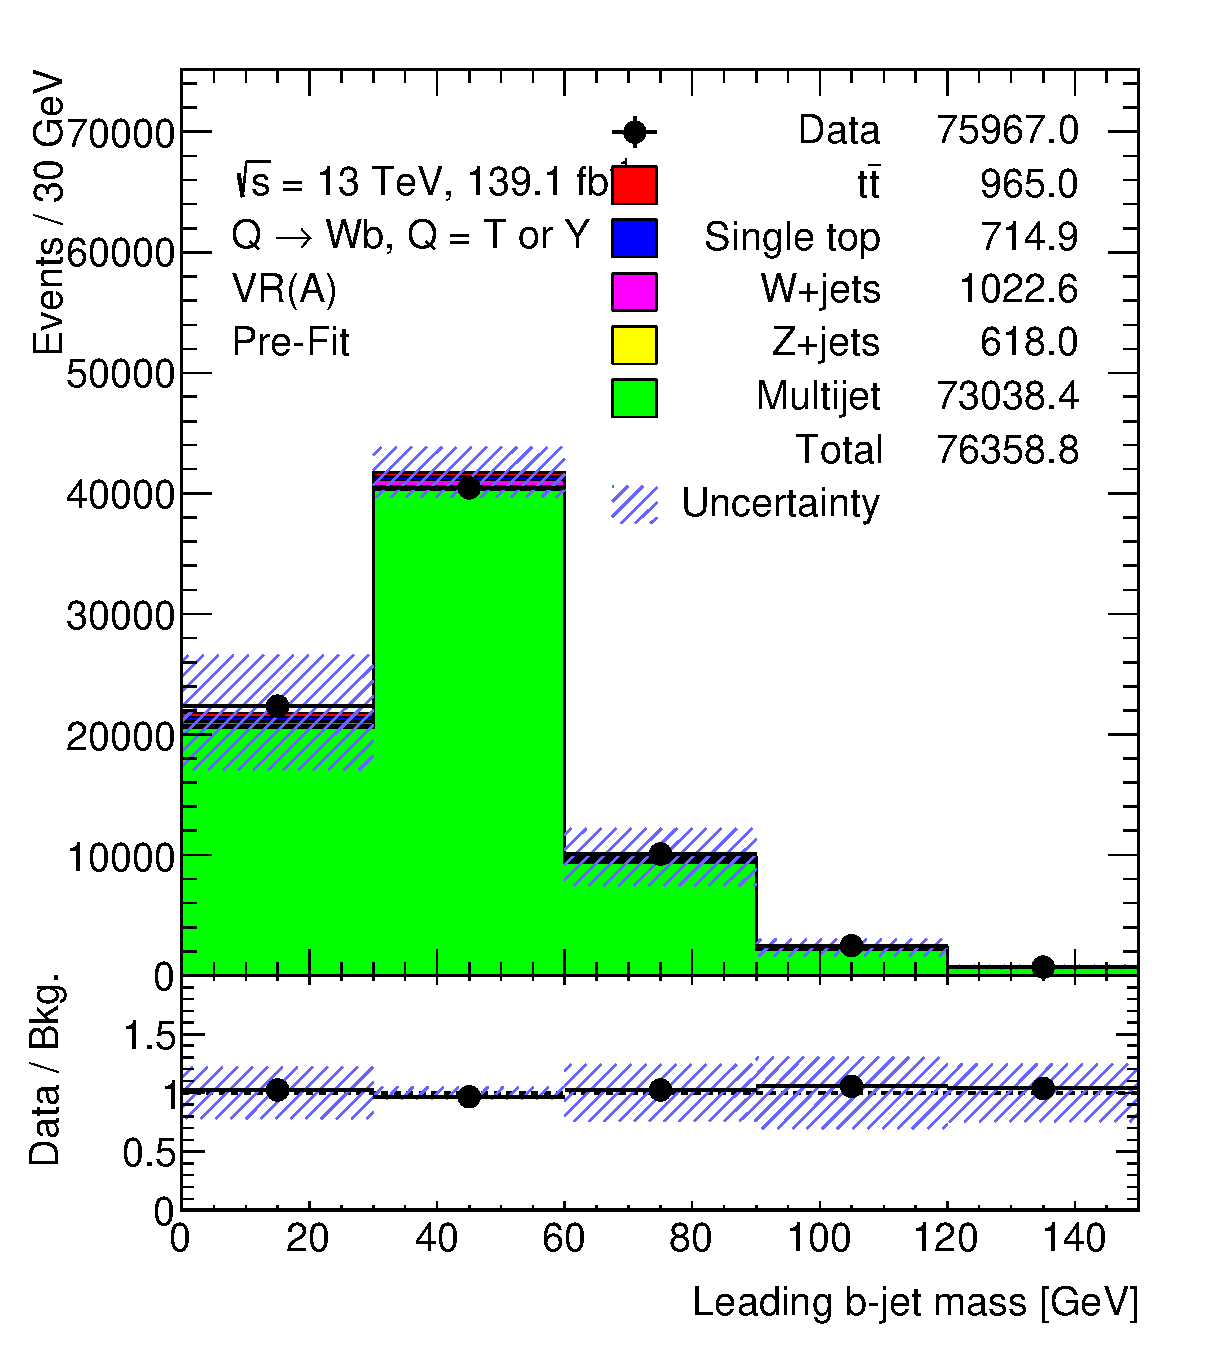
\includegraphics[width=\linewidth,height=\textheight,keepaspectratio]{VR_B_jet_m.eps}
		\caption{}
		\label{fig:results:estimation:jet_m}
	\end{subfigure}
	\caption{Estimated multijet background from the ABCD method including all the uncertainties in the validation region. The distributions include (a) $p_{\text{T}}$ of $W$-tagged large-$R$ jet, (b) $p_{\text{T}}$ of leading $b$-tagged small-$R$ jet, (c) VLQ mass reconstructed from the kinematics of $W$-tagged large-$R$ jet and leading $b$-tagged small-$R$ jet, (d) $\eta$ distribution of $W$-tagged large-$R$ jet, (e) mass of $W$-tagged large-$R$ jet, and (f) mass of leading $b$-tagged small-$R$ jet.}
	\label{fig:results:estimation}
\end{figure}


%==============================================================================
\section{Performance comparison of two different $W$-taggers}
\label{sec:results:taggers}
%==============================================================================

A performance comparison is evaluated between the choice of the $W$-tagger. As described in section \ref{sec:jetsandtaggers:taggers:twovariable}, the large-$R$ jets also are tagged with two-variable tagger. Then, the entire ABCD method is performed again by using these $W$-tagged jets instead of previously using the three-variable tagger for $W$-tagged jets. While performing the ABCD method, all the other variables and parameters are kept similar to the one in the case of the three-variable tagger. \R is calculated from scaled multijet MC (as described in section \ref{sec:abcd:furtherimprovement:rcorr}) by using the shape method for both the cases. All the uncertainties are calculated in exactly a similar way, how it is calculated in the case of the three-variable tagger. 

Fig.\ \ref{fig:results:taggers} shows all the six the kinematic distributions in the validation region when $W$-tagging is performed by the two-variable tagger. A data/bkg.\ comparison is shown in these distributions where multijet is estimated by the ABCD method. The uncertainties shown in the plots include both statistical and systematics uncertainties which are calculated in a similar way for the two-variable tagger case. One can see more number of events (almost double) in data and estimated multijet event yield, which means that two-variable tagger is tagging the leading large-$R$ jet in more events than the three-variable tagger at the same working point. Also, a similar trend in the uncertainties can be observed in the distributions which has been observed with the three-variable tagger.

Table \ref{table:results:taggers1} shows the event yield of the estimated multijet along with their uncertainties for the $\eta$ distribution of $W$-tagged jet. It is shown for both the multijet estimate when the $W$-tagging is performed by two-variable tagger and three-variable tagger. It can be observed that the multijet (from the ABCD method) plus the contribution from other backgrounds (from the MC simulation) agree well with the data within the described uncertainties for the results from two-variable tagger as well.

\begin{table}[hbt!]
	\centering
	\begin{tabular}{c | c | c } 
		\toprule
		 & Two-variable tagger & Three-variable tagger \\
		\midrule
		Est.\ multijet & $\num{140634} \pm \num{506} \text{ (stat.)} \pm \num{5288} \text{ (sys.)}$ & $\num{72613} \pm \num{290} \text{ (stat.)} \pm \num{3199} \text{ (sys.)}$ \\
		Other bkg.\ & $\num{4210} \pm \num{101} \text{ (stat.)}$ & $\num{3320} \pm \num{95} \text{ (stat.)}$ \\
		\midrule
		\textbf{Data} & \textbf{\num{145892}} & \textbf{\num{75967}} \\
		\bottomrule
	\end{tabular}
	\caption{Result showing the estimated multijet with all the uncertainties in the validation region for the $\eta$ distribution of $W$-tagged jet when two-variable and three-variable tagger are used for $W$-tagging.}
	\label{table:results:taggers1}
\end{table}

Table \ref{table:results:taggers} shows the event yield of the data in different ABCD regions when $W$-tagging is performed both by two-variable tagger and three-variable tagger. Since the ABCD method is a data-driven method and one of the assumptions of this method as described in section \ref{sec:abcd:method}, is that there should be enough number of data events in the control region to extrapolate the background behaviour precisely in the distributions of the validation region. That means, more statistics in the data in region B, C and D can extrapolate the multijet background precisely. In the table, it can be seen clearly that when the $W$-tagging is performed by the three-variable tagger, there are more data events in the control regions (except region D). That is why three-variable tagger is used for $W$-tagging in the final estimate of the multijet background. Moreover, the three-variable tagger is developed to be sensitive to the QCD rejection, which has higher QCD rejection than the two-variable tagger.


\begin{table}[hbt!]
	\centering
	\begin{tabular}{c | c | c | c | c | c | c} 
		\toprule
		Event yield in data & SR & VR & \multicolumn{4}{c}{CR} \\ \cline{2-7}
		& Region A1 & Region A & Region B & Region C & Region D & Region D1 \\
		\midrule
		Two-variable tagger & - & \num{145892} & \num{267559} & \num{478436} & \num{196851} & \num{11625} \\
		Three-variable tagger & - & \num{75967} & \num{365089} & \num{605052} & \num{95173} & \num{18719} \\
		\bottomrule
	\end{tabular}
	\caption{Result showing the event yields of the data in all the ABCD regions when $W$-tagging is performed by both two-variable and three-variable tagger.}
	\label{table:results:taggers}
\end{table}

\begin{figure}[hbt!]
	\centering
	\graphicspath{{figs/chapter6/twovariable/}}
	\begin{subfigure}{.35\textwidth}
		\centering
		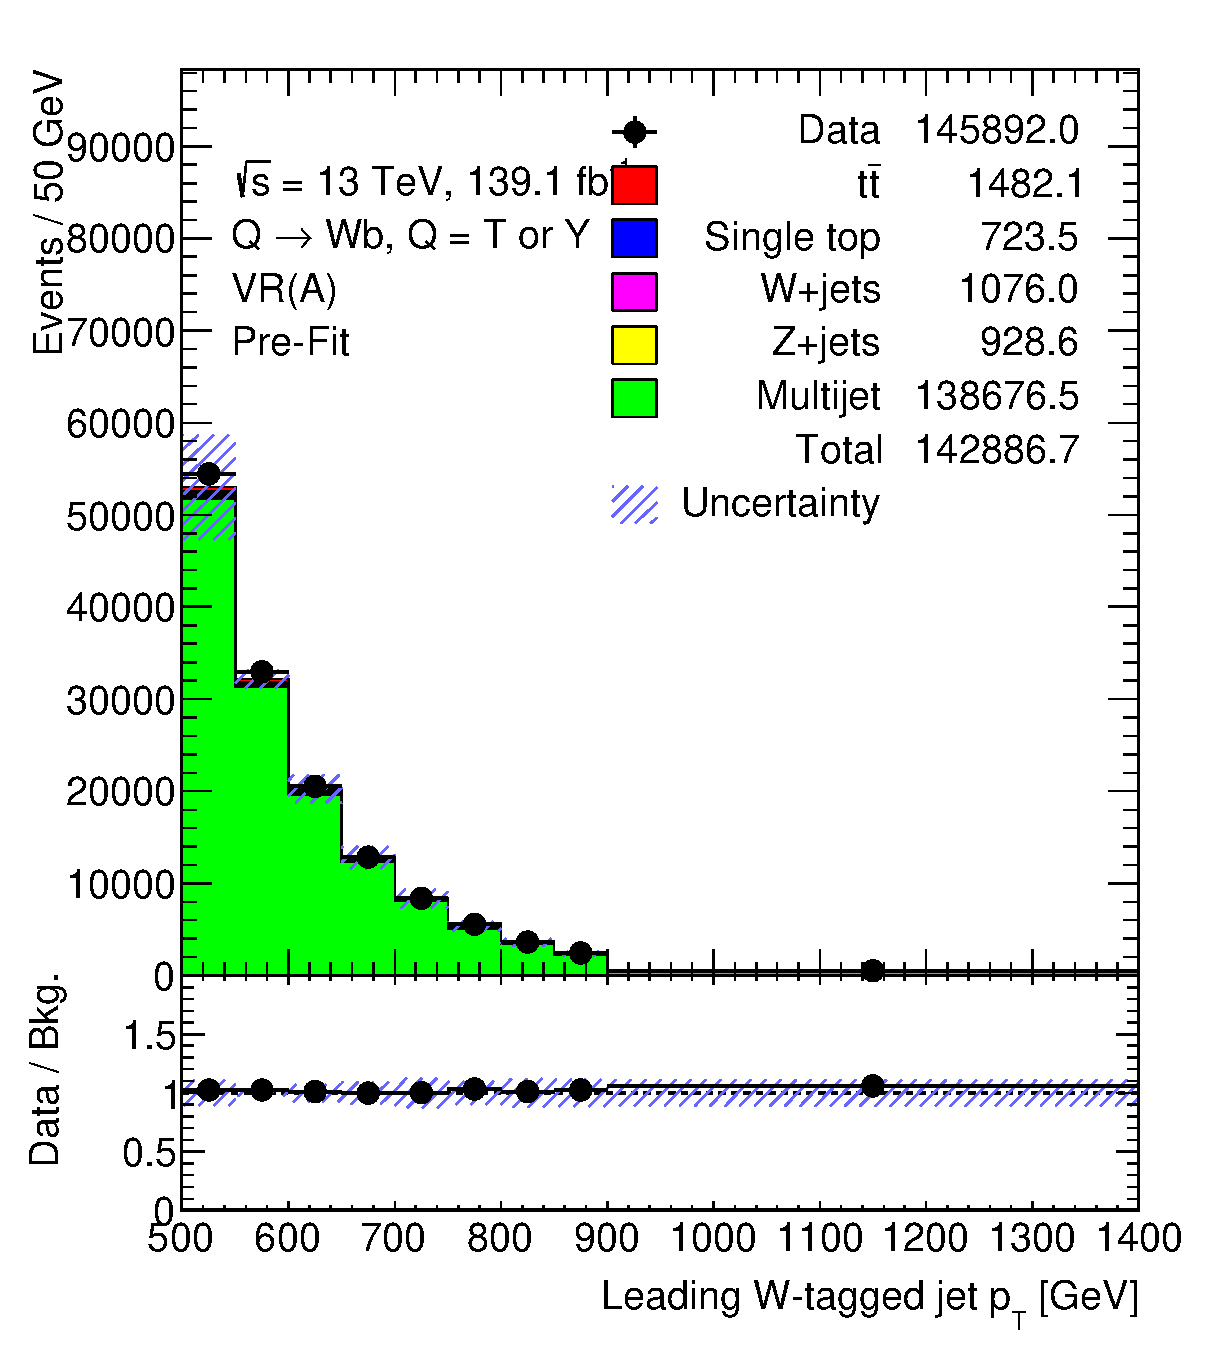
\includegraphics[width=\linewidth,height=\textheight,keepaspectratio]{VR_B_ljet_pt.eps}
		\caption{}
		\label{fig:results:taggers:ljet_pt}
	\end{subfigure}\hspace{0.6cm}
	\begin{subfigure}{.35\textwidth}
		\centering
		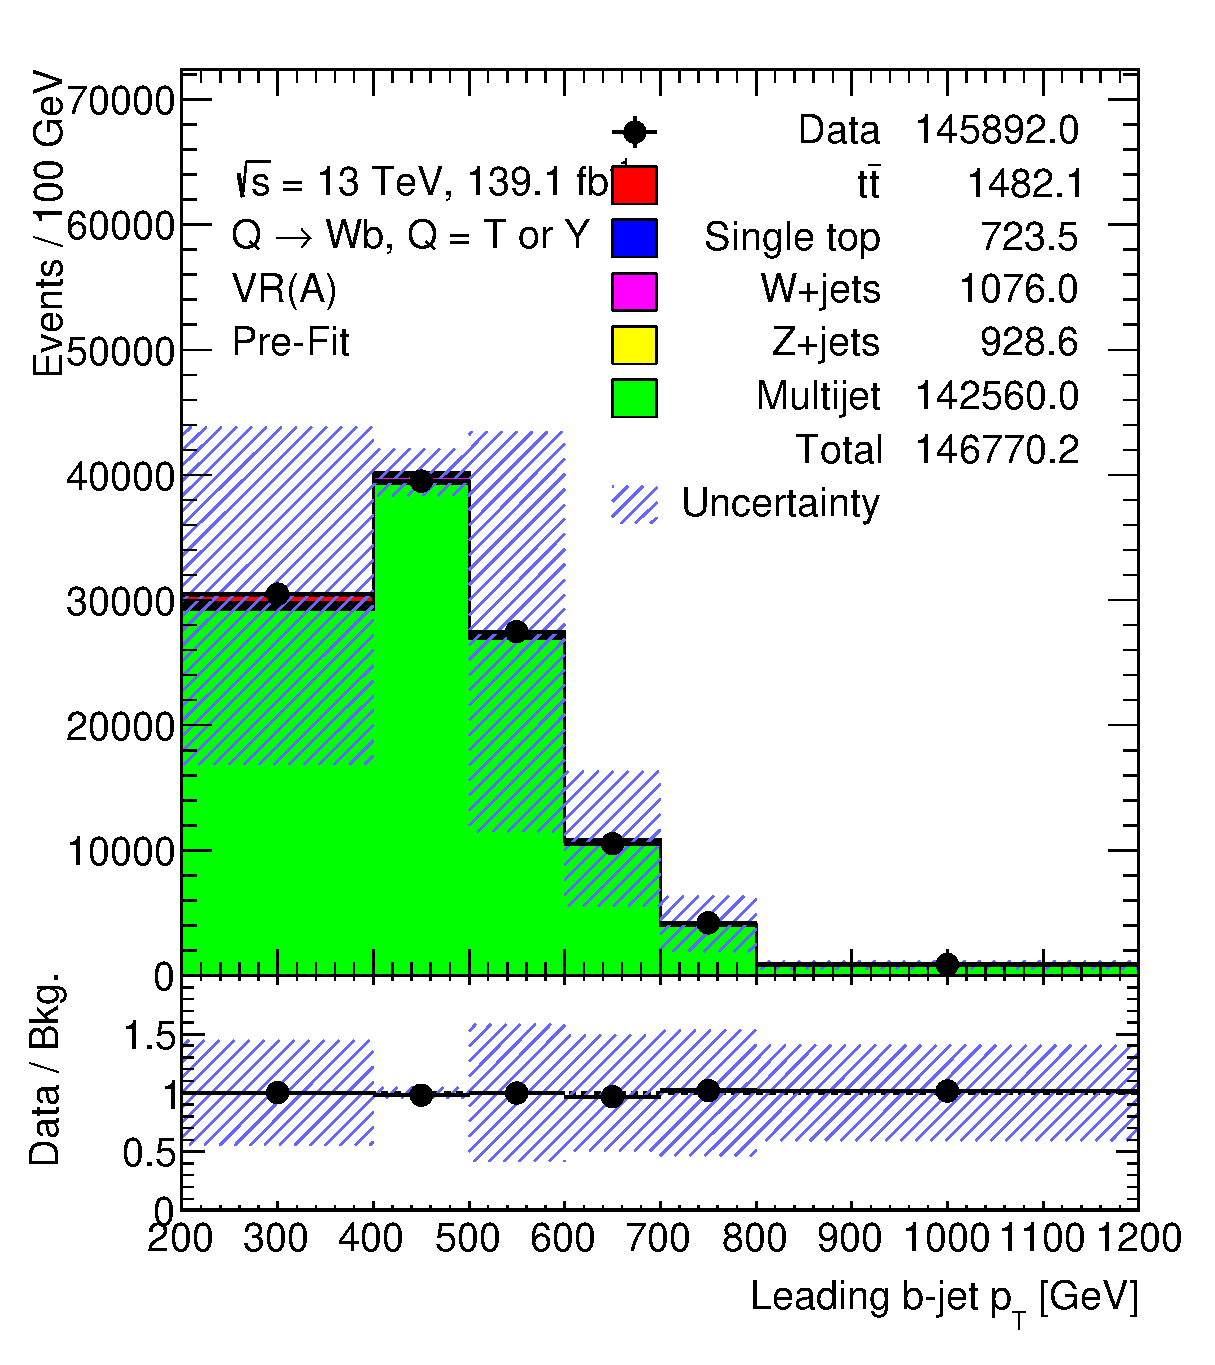
\includegraphics[width=\linewidth,height=\textheight,keepaspectratio]{VR_B_jet_pt.eps}
		\caption{}
		\label{fig:results:taggers:jet_pt}
	\end{subfigure}
	\begin{subfigure}{.35\textwidth}
		\centering
		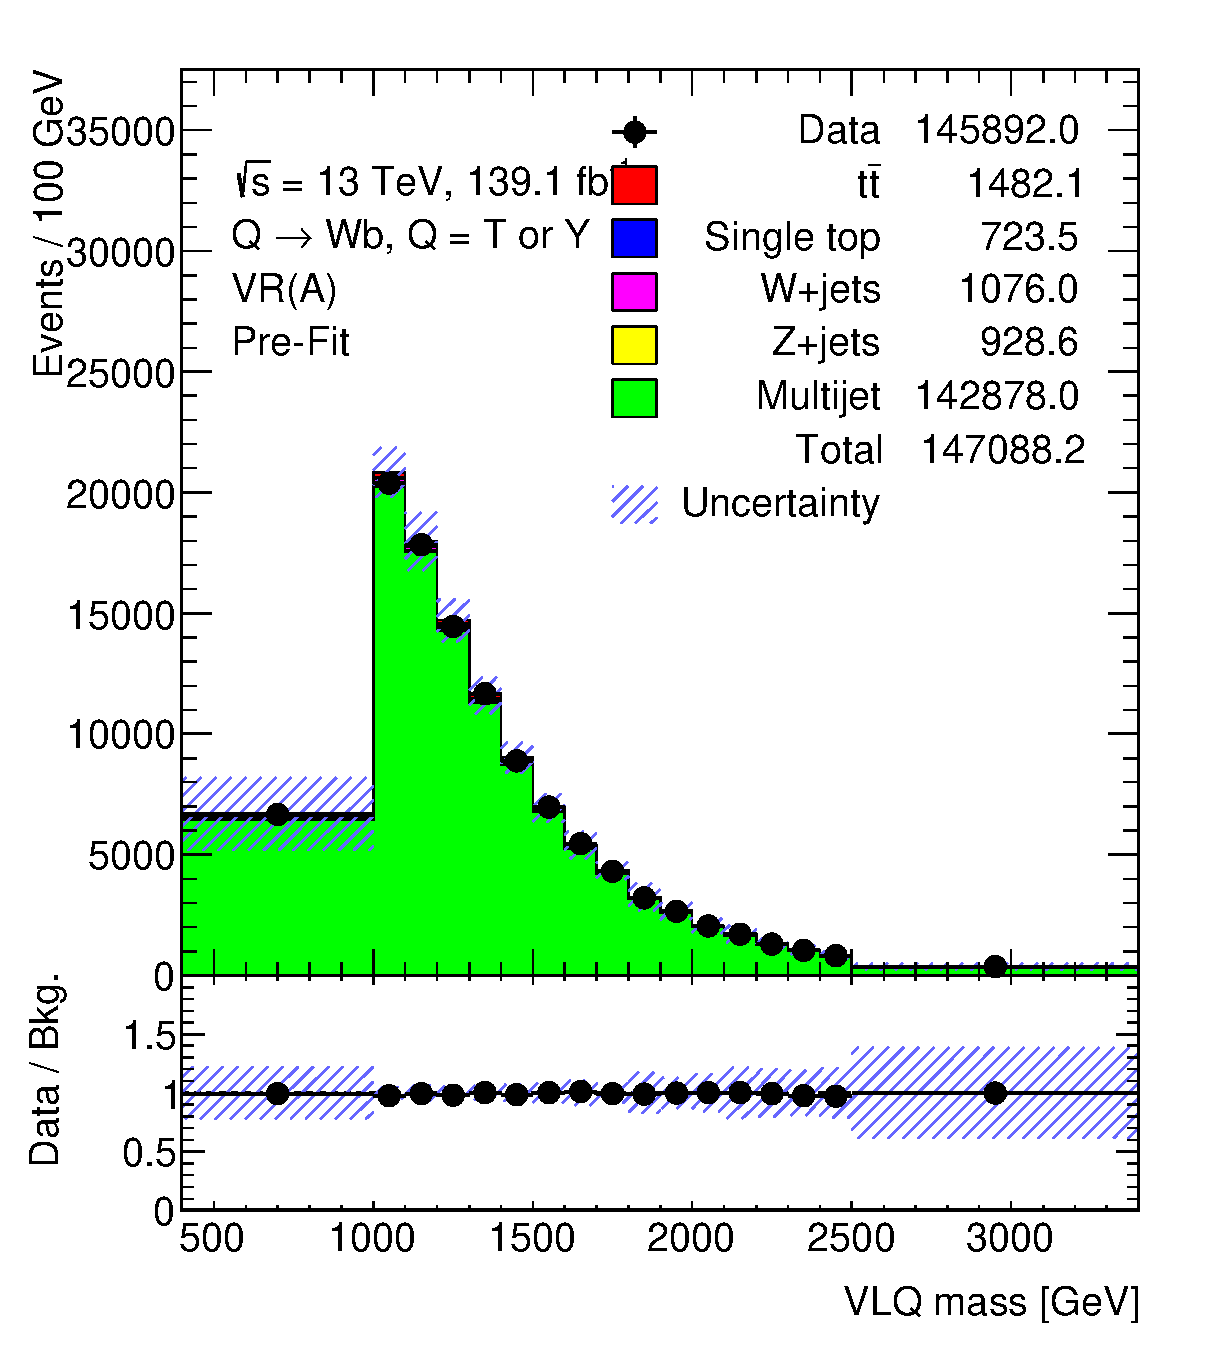
\includegraphics[width=\linewidth,height=\textheight,keepaspectratio]{VR_B_VLQM.eps}
		\caption{}
		\label{fig:results:taggers:VLQM}
	\end{subfigure}\hspace{0.6cm}
	\begin{subfigure}{.35\textwidth}
		\centering
		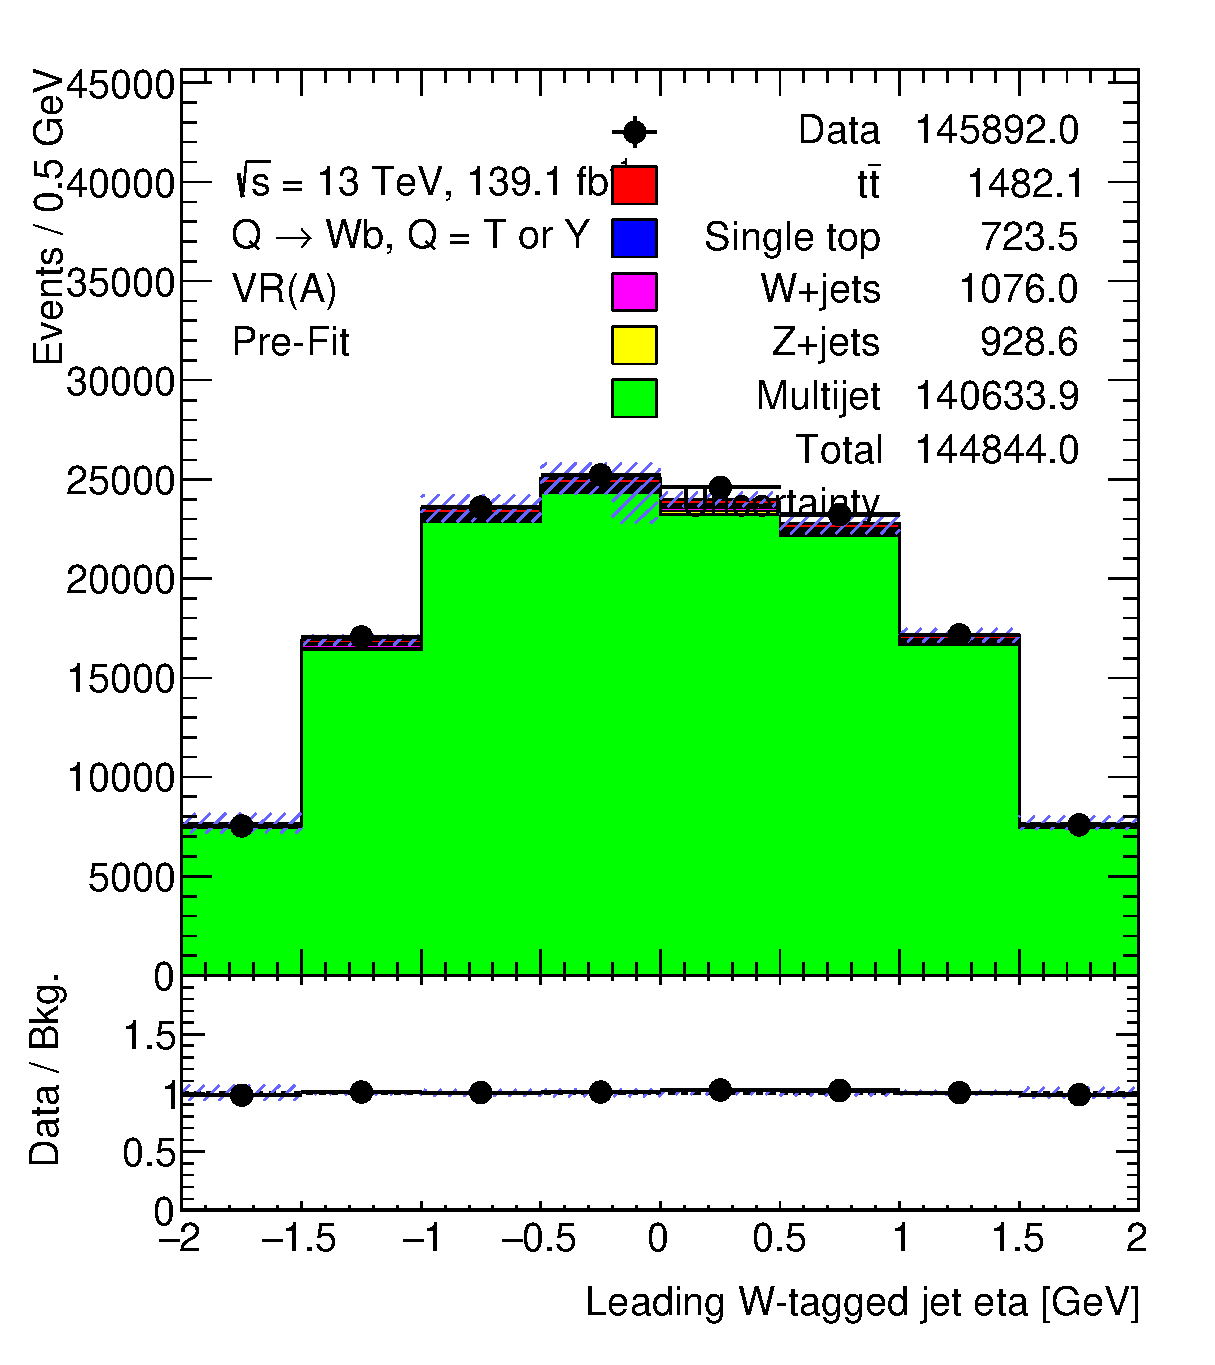
\includegraphics[width=\linewidth,height=\textheight,keepaspectratio]{VR_B_ljet_eta.eps}
		\caption{}
		\label{fig:results:taggers:ljet_eta}
	\end{subfigure}
	\begin{subfigure}{.35\textwidth}
		\centering
		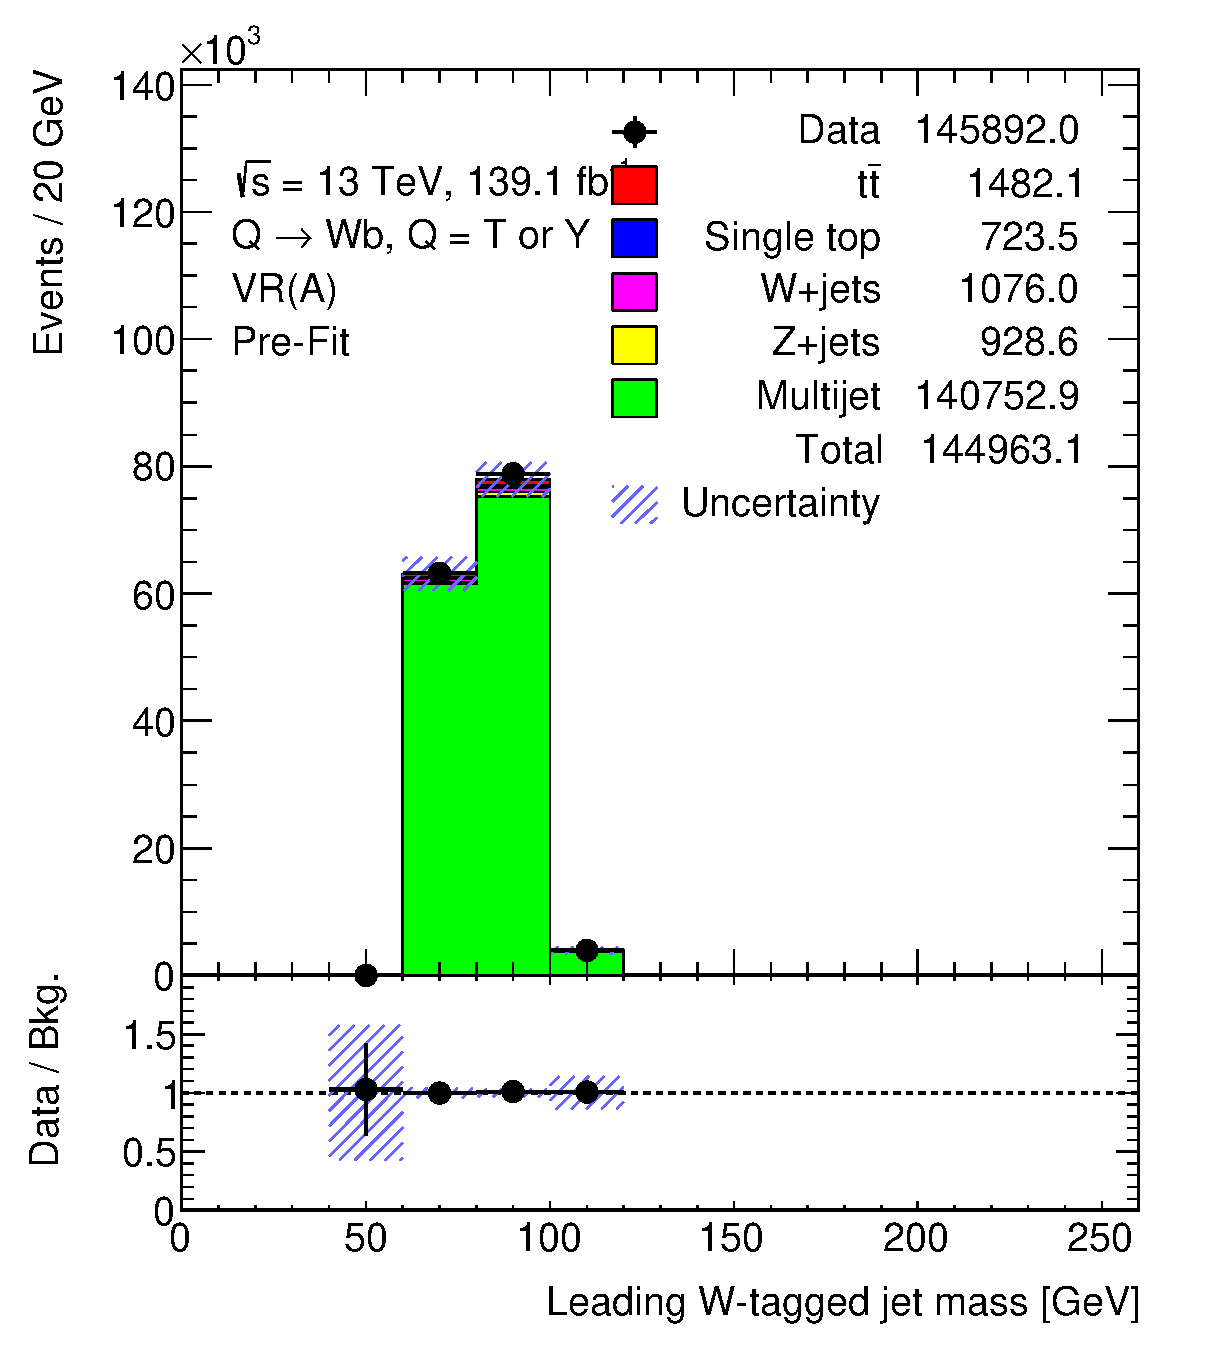
\includegraphics[width=\linewidth,height=\textheight,keepaspectratio]{VR_B_ljet_m.eps}
		\caption{}
		\label{fig:results:taggers:ljet_m}
	\end{subfigure}\hspace{0.6cm}
	\begin{subfigure}{.35\textwidth}
		\centering
		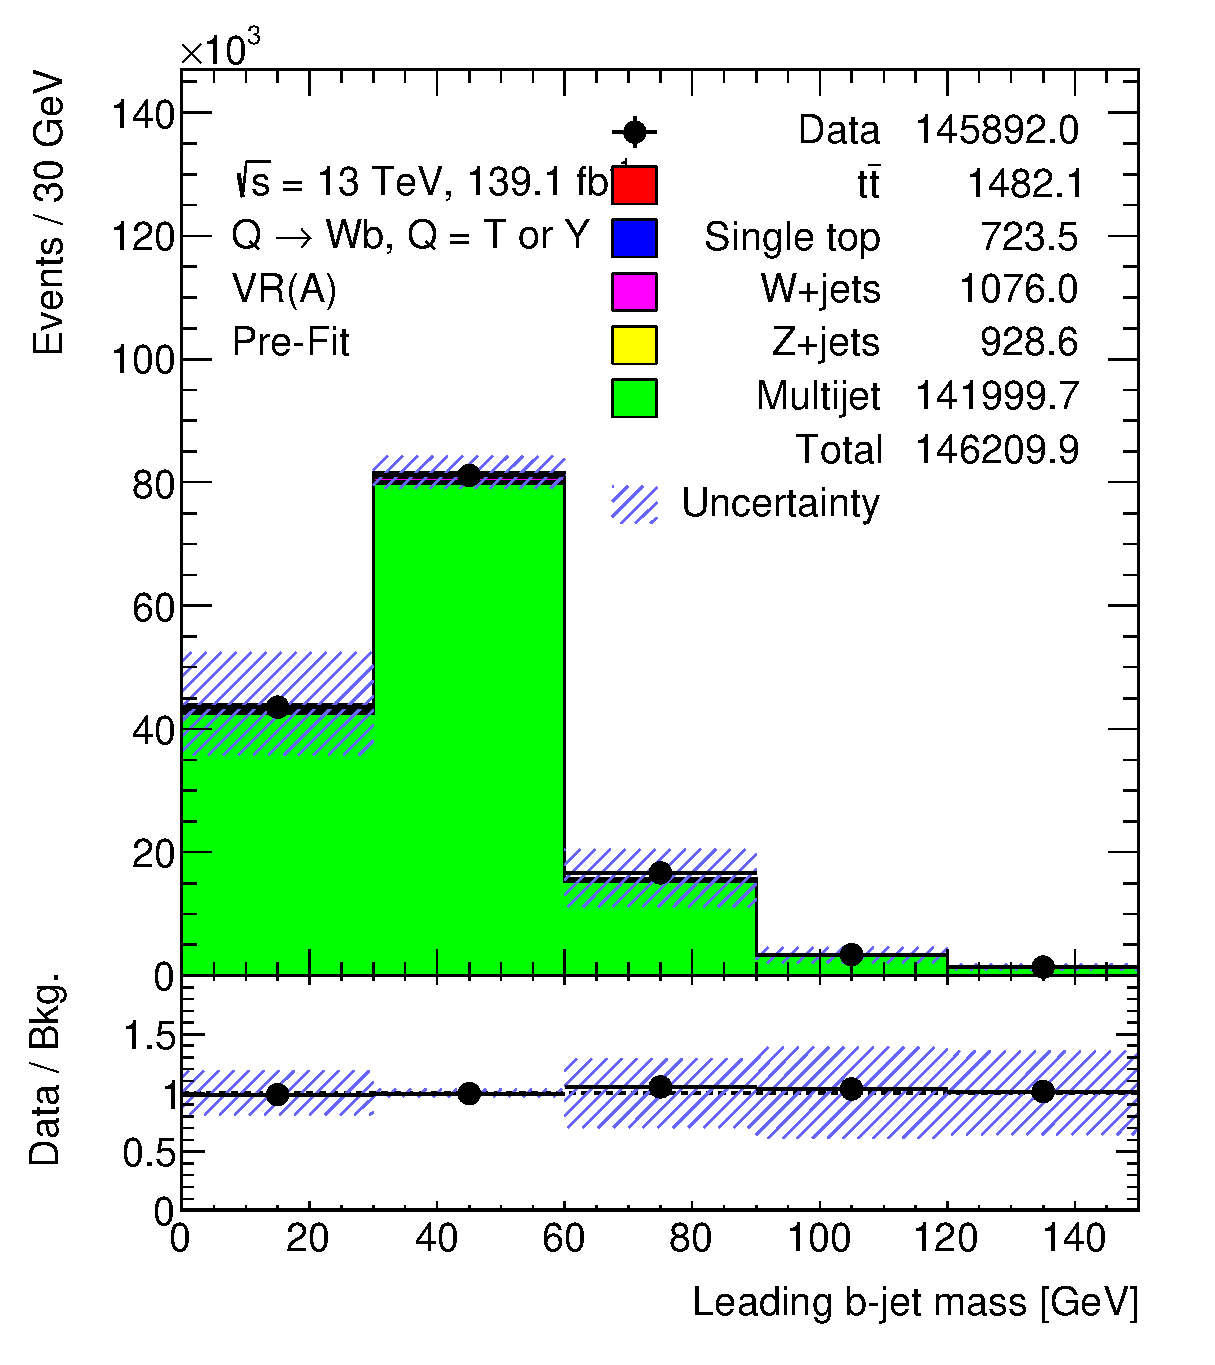
\includegraphics[width=\linewidth,height=\textheight,keepaspectratio]{VR_B_jet_m.eps}
		\caption{}
		\label{fig:results:taggers:jet_m}
	\end{subfigure}
	\caption{Results when $W$-tagging is performed by using the two-variable tagger in the estimate of multijet background from the ABCD method including all the uncertainties in the validation region. The distributions include (a) $p_{\text{T}}$ of $W$-tagged large-$R$ jet, (b) $p_{\text{T}}$ of leading $b$-tagged small-$R$ jet, (c) VLQ mass reconstructed from the kinematics of $W$-tagged large-$R$ jet and leading $b$-tagged small-$R$ jet, (d) $\eta$ distribution of $W$-tagged large-$R$ jet, (e) mass of $W$-tagged large-$R$ jet, and (f) mass of leading $b$-tagged small-$R$ jet.}
	\label{fig:results:taggers}
\end{figure}


%==============================================================================
\section{Performance comparison of two different jet collections}
\label{sec:results:jetcollections}
%==============================================================================
A performance comparison is also evaluated between the choice of the jet collection for small-$R$ jets. As described in section \ref{sec:jetsandtaggers:jets:topo}, the topo-cluster jet collection is also used for small-$R$ jets which are calibrated to electromagnetic scale and the $b$-tagging is performed on these small-$R$ jets. Another difference is that there are different versions of \textsc{AnalysisTop}~\cite{analysistop} used for EMTopo and particle flow jets, e.g.\ \textsc{AnalysisTop 21.2.84}~\cite{analysistop} is used for EMTopo jet collection and \textsc{AnalysisTop 21.2.92}~\cite{analysistop} is used for particle flow jet collections. 

The entire ABCD method is performed again by using these $b$-tagged jets (where the small-$R$ jets are from EMTopo jet collections) instead of previously using the $b$-tagged jets from particle flow jet collection. While performing the ABCD method, all the other variables and parameters are kept similar to the one in the particle flow case. \R is calculated from scaled multijet MC (as described in section \ref{sec:abcd:furtherimprovement:rcorr}) by using the shape method for both the cases. All the uncertainties are calculated in exactly a similar way, how it is calculated in the case of the particle flow jet collection for small-$R$ jets.  

Fig.\ \ref{fig:results:jetcollections} shows the kinematic distributions in the validation region when the EMTopo jet collection is used for small-$R$ jets. A data/bkg.\ comparison is shown in these distributions where multijet is estimated by the ABCD method. One can see less number of events in data and estimated multijet event yield. The uncertainties shown in the plots include both statistical and systematic uncertainties which are already discussed for the particle flow case.

Table \ref{table:results:jetcollections1} shows the event yield of the estimated multijet along with their uncertainties for the $\eta$ distribution of $W$-tagged jet. It is shown for both the multijet estimate when the small-$R$ jets are from EMTopo jets collection and particle flow jet collection. Here, $W$-tagging is performed by three-variable tagger in both the cases. It can be observed that the multijet (from the ABCD method) plus the contribution from other backgrounds (from the MC simulation) agree well with the data within the described uncertainties for the results from EMTopo jet collection as well. But the particle flow jet collection gives better statistics and shows better agreement with the data. 

\begin{table}[hbt!]
	\centering
	\begin{tabular}{c | c | c } 
		\toprule
		& EMTopo jets & Particle flow jets \\
		\midrule
		Est.\ multijet & $\num{64212} \pm \num{229} \text{ (stat.)} \pm \num{3981} \text{ (sys.)}$ & $\num{72613} \pm \num{290} \text{ (stat.)} \pm \num{3199} \text{ (sys.)}$ \\
		Other bkg.\ & $\num{2981} \pm \num{89} \text{ (stat.)}$ & $\num{3320} \pm \num{95} \text{ (stat.)}$ \\
		\midrule
		\textbf{Data} & \textbf{\num{66708}} & \textbf{\num{75967}} \\
		\bottomrule
	\end{tabular}
	\caption{Result showing the estimated multijet with all the uncertainties in the validation region for the $\eta$ distribution of $W$-tagged jet when EMTopo and particle flow jet collections are used for small-$R$ jets.}
	\label{table:results:jetcollections1}
\end{table}

Table \ref{table:results:jetcollections} shows the event yield of the data in different ABCD regions when both EMTopo and particle flow jet collections are used one-by-one for small-$R$ jets.
From the event yield in the data, one can see that there is more number of data events in the control regions when EMTopo jet collection is used for small-$R$ jets than the particle flow jet collection. 

\begin{table}[hbt!]
	\centering
	\begin{tabular}{c | c | c | c | c | c | c} 
		\toprule
		Event yield in data & SR & VR & \multicolumn{4}{c}{CR} \\ \cline{2-7}
		& Region A1 & Region A & Region B & Region C & Region D & Region D1 \\
		\midrule
		EMTopo jets & - & \num{66708} & \num{1590130} & \num{4313450} & \num{100573} & \num{19911} \\
		Particle flow jets & - & \num{75967} & \num{365089} & \num{605052} & \num{95173} & \num{18719} \\
		\bottomrule
	\end{tabular}
	\caption{Result showing the event yields of the data in all the ABCD regions when EMTopo and particle flow jet collections are used for small-$R$ jets.}
	\label{table:results:jetcollections}
\end{table}


\begin{figure}[hbt!]
	\centering
	\graphicspath{{figs/chapter6/topo/}}
	\begin{subfigure}{.35\textwidth}
		\centering
		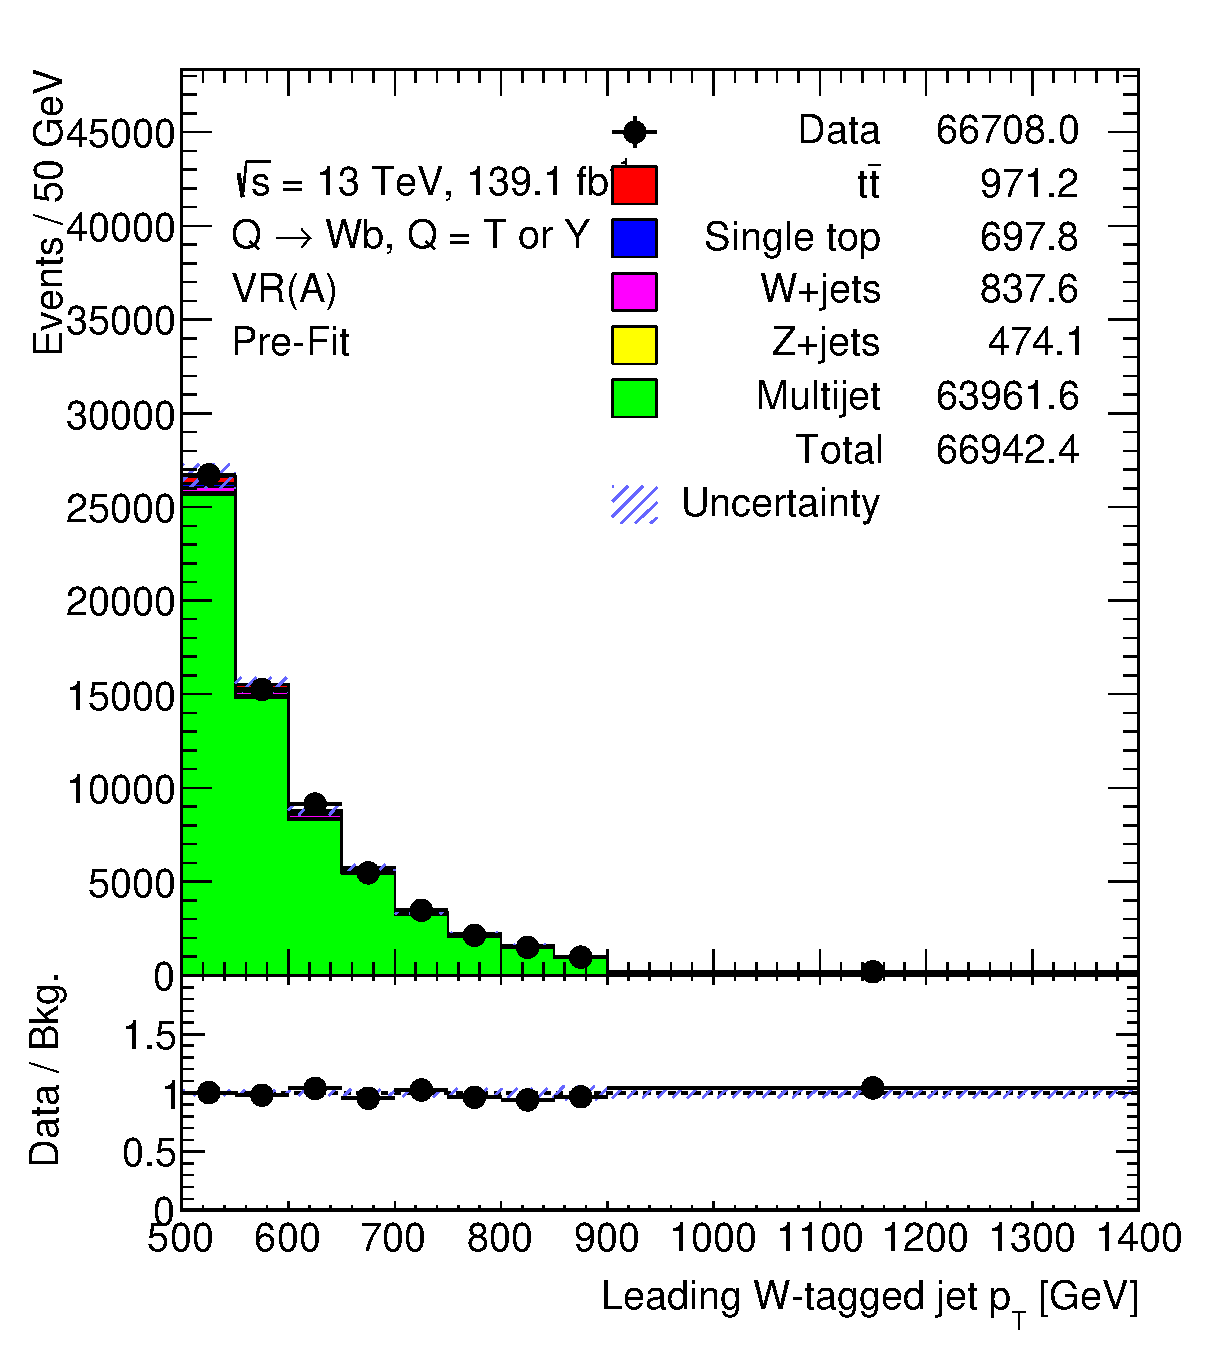
\includegraphics[width=\linewidth,height=\textheight,keepaspectratio]{VR_B_ljet_pt.eps}
		\caption{}
		\label{fig:results:jetcollections:ljet_pt}
	\end{subfigure}\hspace{0.6cm}
	\begin{subfigure}{.35\textwidth}
		\centering
		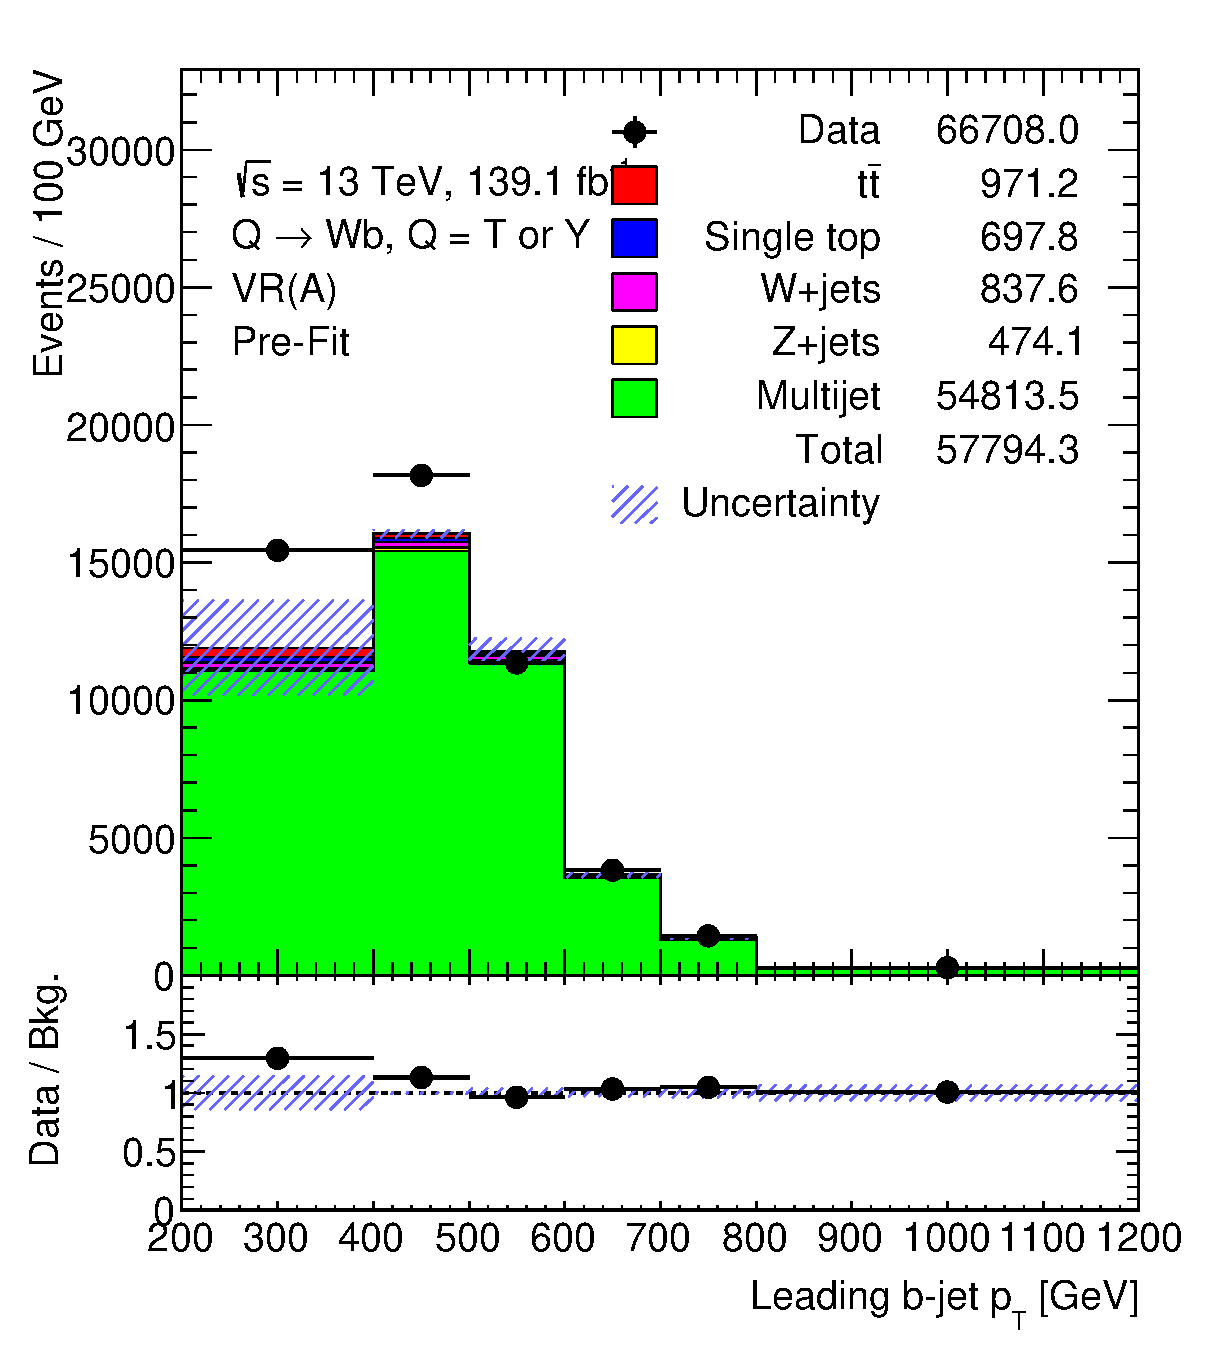
\includegraphics[width=\linewidth,height=\textheight,keepaspectratio]{VR_B_jet_pt.eps}
		\caption{}
		\label{fig:results:jetcollections:jet_pt}
	\end{subfigure}
	\begin{subfigure}{.35\textwidth}
		\centering
		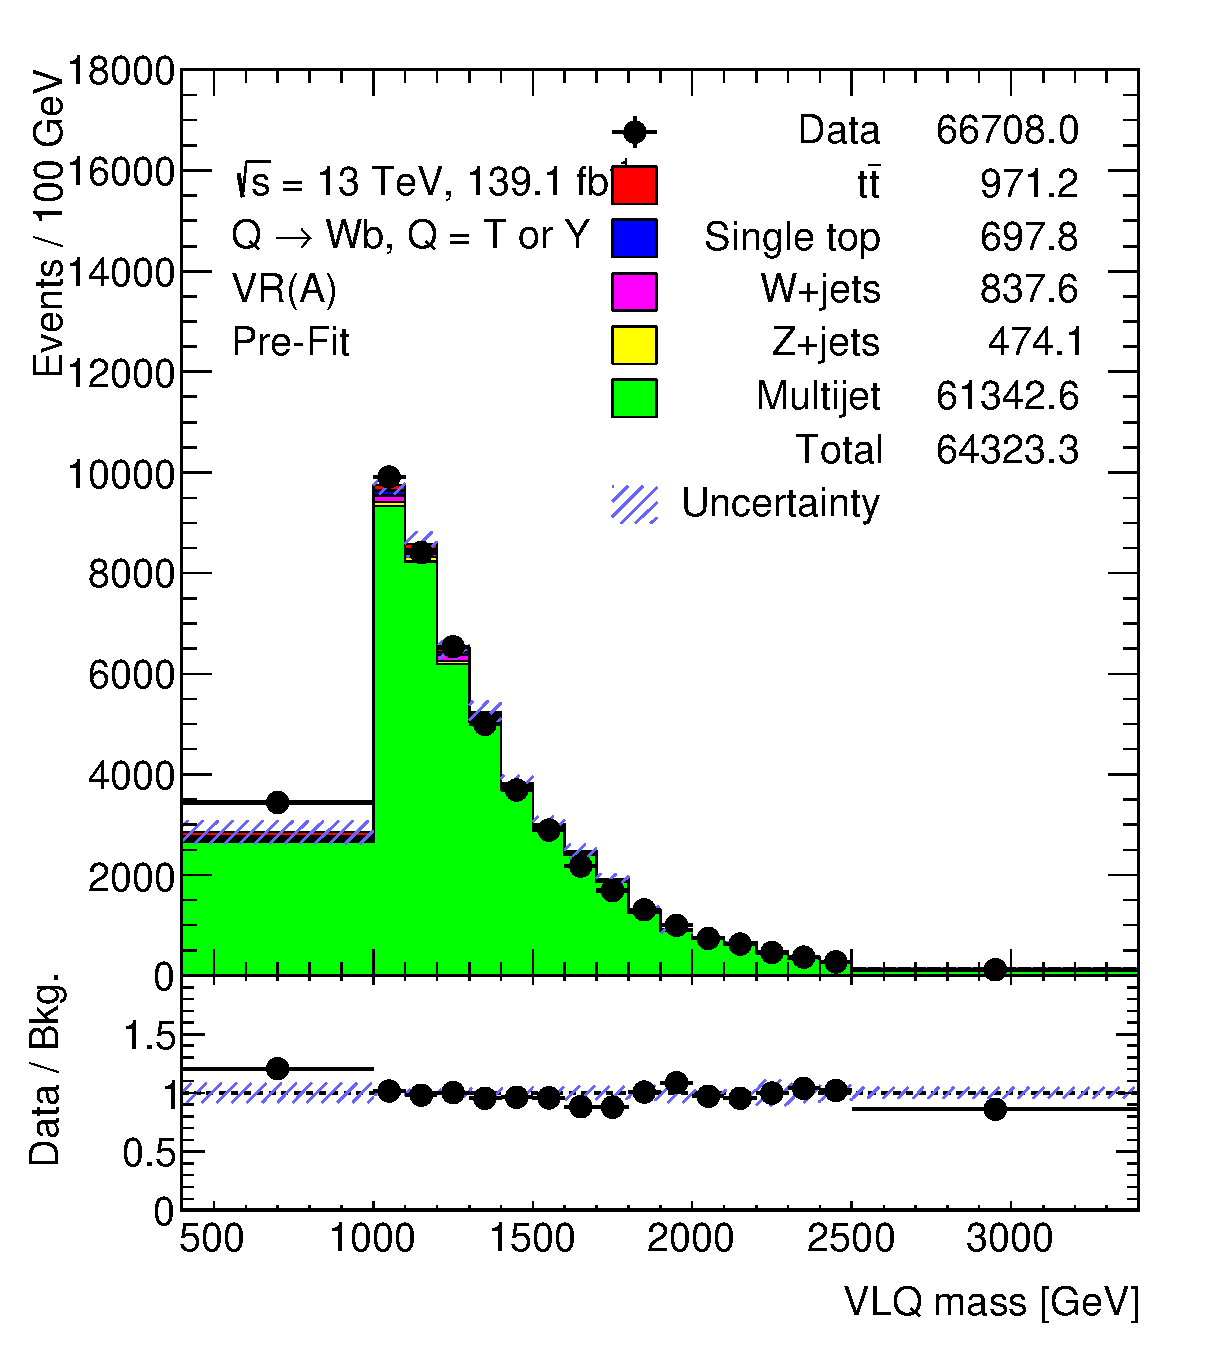
\includegraphics[width=\linewidth,height=\textheight,keepaspectratio]{VR_B_VLQM.eps}
		\caption{}
		\label{fig:results:jetcollections:VLQM}
	\end{subfigure}\hspace{0.6cm}
	\begin{subfigure}{.35\textwidth}
		\centering
		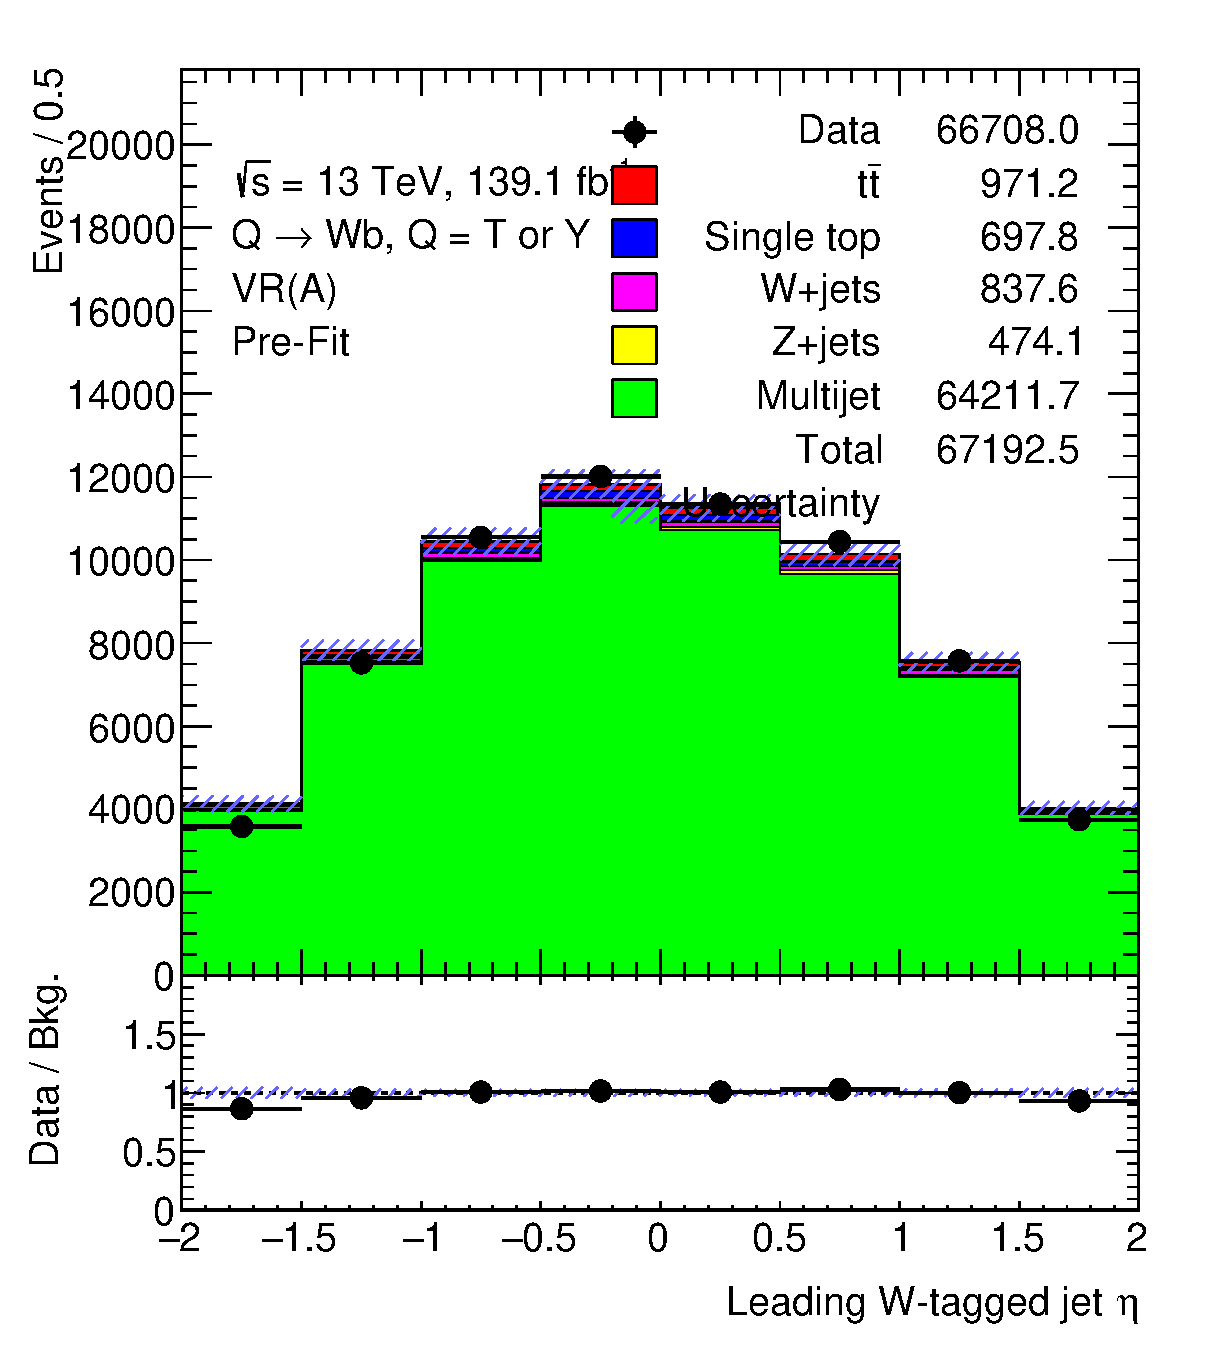
\includegraphics[width=\linewidth,height=\textheight,keepaspectratio]{VR_B_ljet_eta.eps}
		\caption{}
		\label{fig:results:jetcollections:ljet_eta}
	\end{subfigure}
	\begin{subfigure}{.35\textwidth}
		\centering
		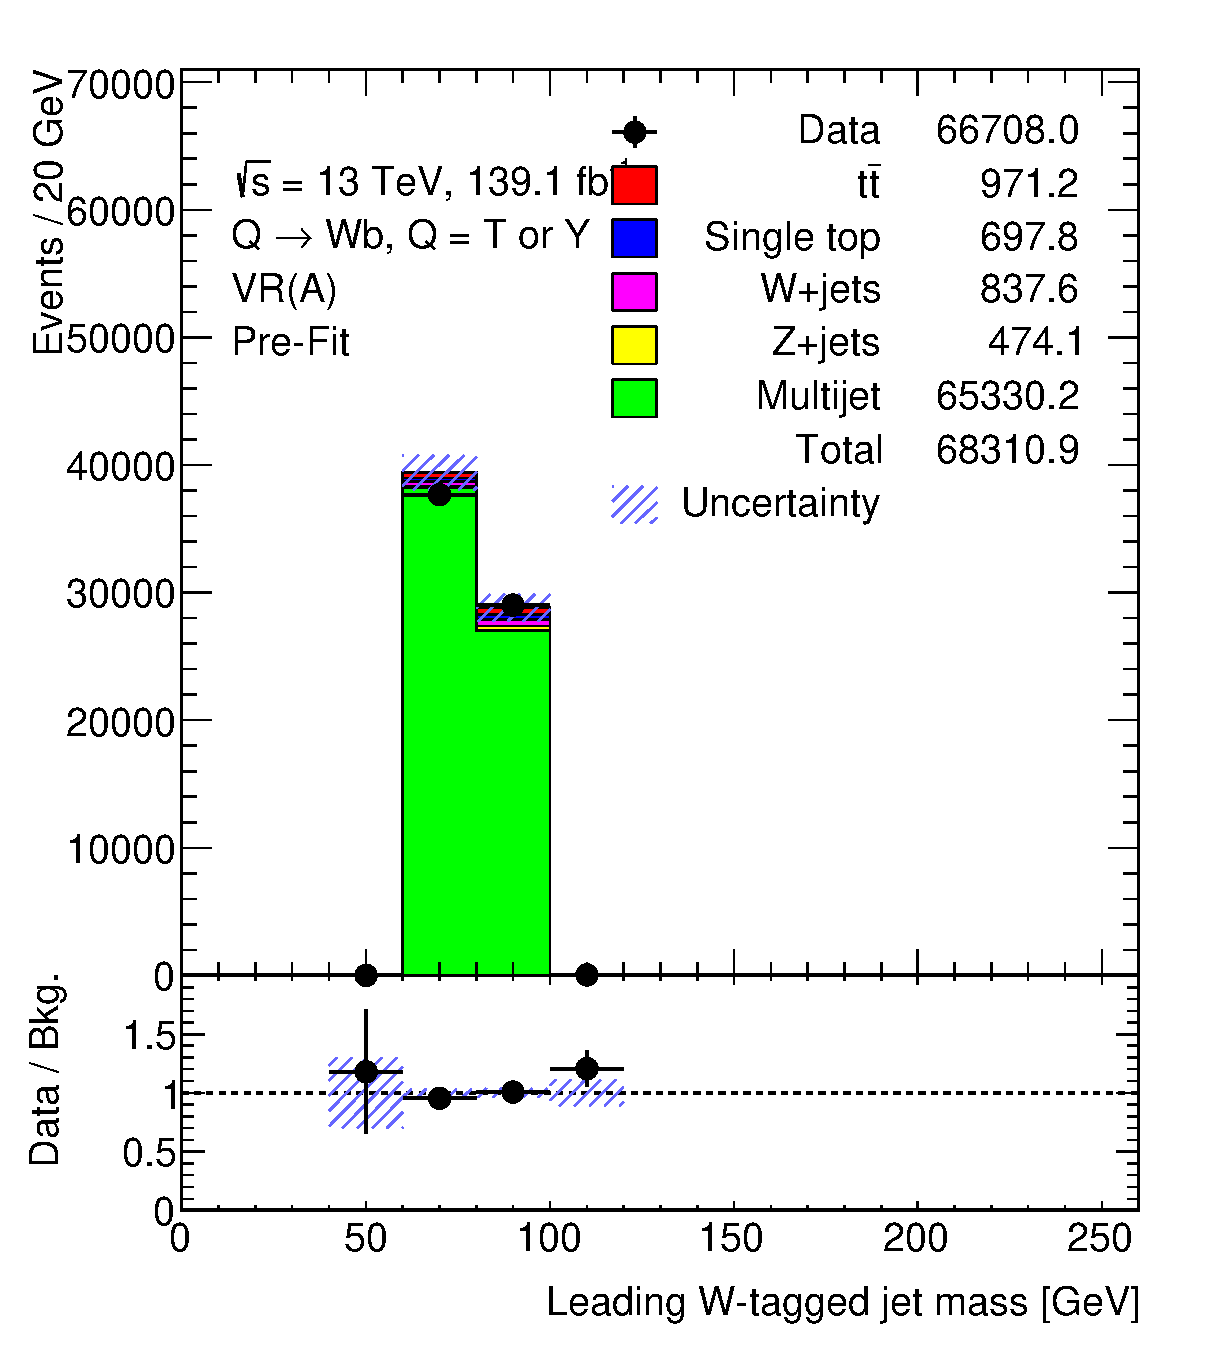
\includegraphics[width=\linewidth,height=\textheight,keepaspectratio]{VR_B_ljet_m.eps}
		\caption{}
		\label{fig:results:jetcollections:ljet_m}
	\end{subfigure}\hspace{0.6cm}
	\begin{subfigure}{.35\textwidth}
		\centering
		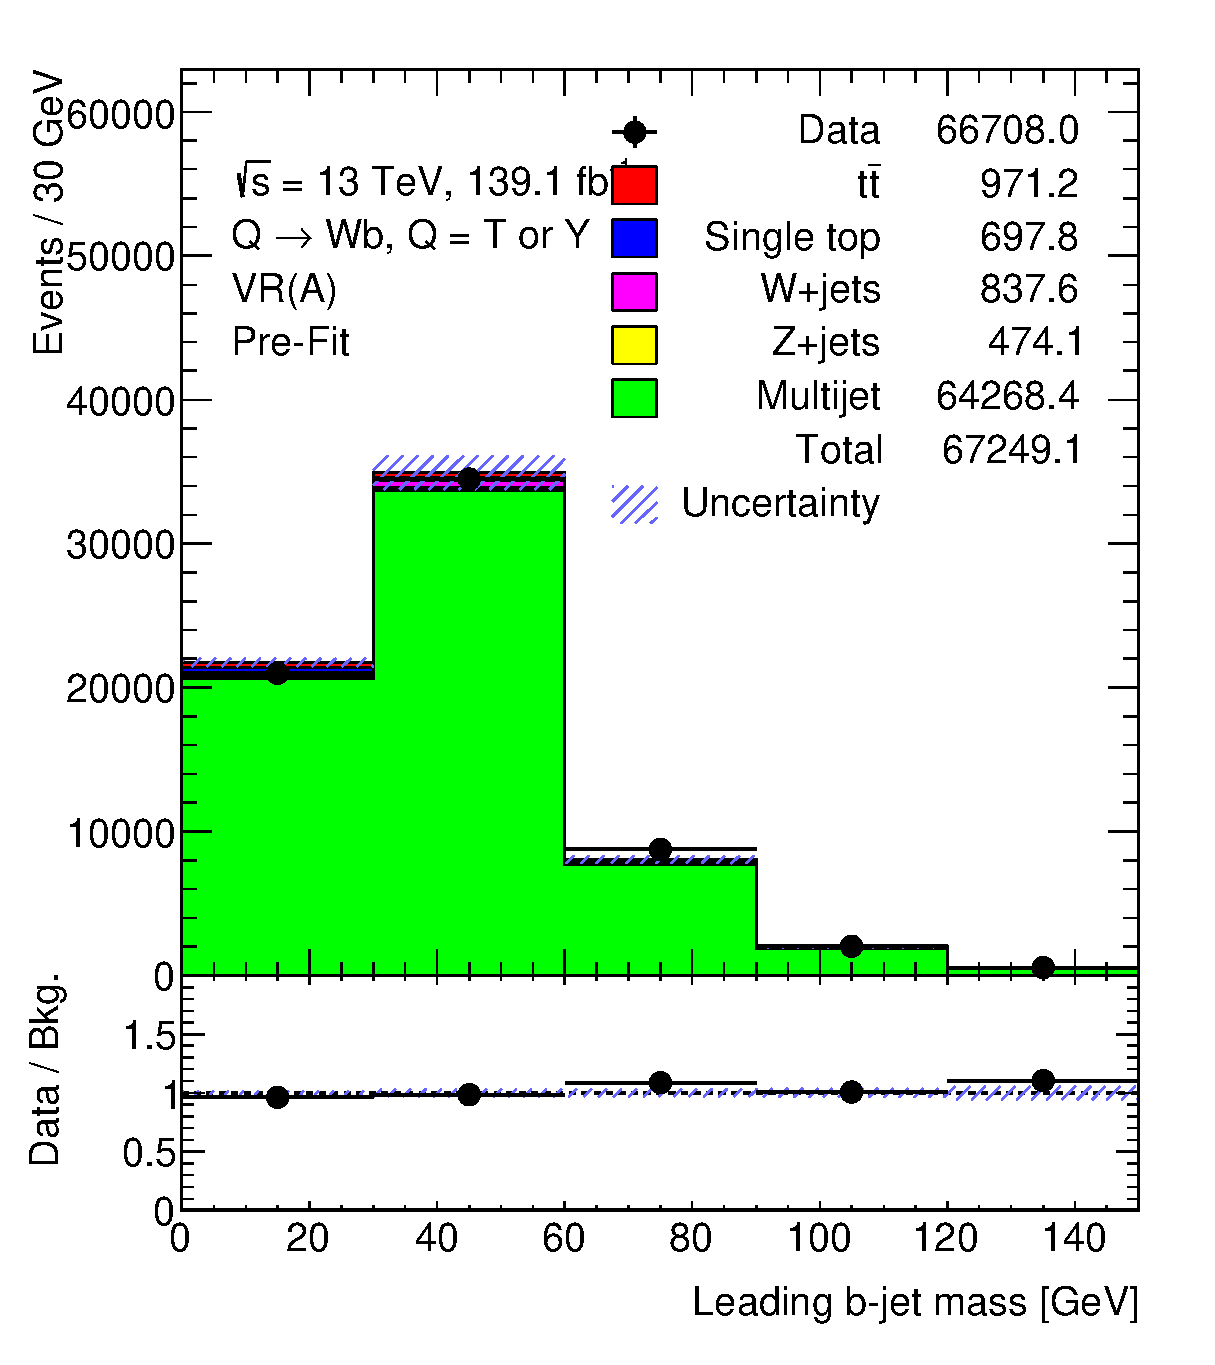
\includegraphics[width=\linewidth,height=\textheight,keepaspectratio]{VR_B_jet_m.eps}
		\caption{}
		\label{fig:results:jetcollections:jet_m}
	\end{subfigure}
	\caption{Results when EMTopo jet collection is used for for small-$R$ jets in the estimate of multijet background from the ABCD method including all the uncertainties in the validation region. The distributions include (a) $p_{\text{T}}$ of $W$-tagged large-$R$ jet, (b) $p_{\text{T}}$ of leading $b$-tagged small-$R$ jet, (c) VLQ mass reconstructed from the kinematics of $W$-tagged large-$R$ jet and leading $b$-tagged small-$R$ jet, (d) $\eta$ distribution of $W$-tagged large-$R$ jet, (e) mass of $W$-tagged large-$R$ jet, and (f) mass of leading $b$-tagged small-$R$ jet.}
	\label{fig:results:jetcollections}
\end{figure}



%%% Local Variables: 
%%% mode: latex
%%% TeX-master: "mythesis"
%%% End: 